\section{The HHL Algorithm} \label{the_hhl_algorithm}

The currently asymptotically best classical method known for solving SLEs is the conjugate gradient method, which runs in worst case time \(\onot(N s \sqrt{\kappa} \log_2(1/\varepsilon))\), as described in \cite[complexity analysis on pp. 37-38]{Richard1994} or \cite[pp. 279-306]{Lyche}. Here, \(\varepsilon \in \mathbb{R}_{> 0}\) is the error cap, \(\kappa \in \mathbb{R}_{\geq 1}\) the condition number of the input \(N \times N\) matrix, where \(N \in \mathbb{N}_{\geq 1}\), and \(s \in \mathbb{N}\) is the sparsity as in \Cref{sparse_and_efficiently_row_computable_matrices}, assuming that the matrix is efficiently row-computable. In many practical cases, the given matrix has about \(\onot(\sqrt{N})\) non-zero entries, for which the algorithm yields a runtime of about \(\onot(N^{3/2} \sqrt{\kappa})\), ignoring the complexity factor for keeping the error low. In 2008, the researchers Harrow, Hassidim and Lloyd (HHL) described a quantum algorithmic approach to solving SLEs. In this section, we will give a rigorous description of the HHL algorithm, along with a rework of the original analysis. The original formulation can be found in \cite{Harrow2008}. We will draw a lot of information from the alternative, more comprehensive formulation presented by Dervovic et al. in \cite[pp. 28-42]{Dervovic2018} as well. Our contribution lies in the explicit description of the auxiliary procedures, such as the initialization of a helper state and a description on three-dimensional rotations, as well as more explicit runtime and error bounds. Most of these helper algorithms have been elaborated in \Cref{extensions_of_the_common_quantum_algorithmic_toolbox}.

\subsection{Problem Description and Assumptions \draftcommentgreen{DONE}} \label{hhl_problem_description_and_assumptions}

Starting off, let us pay attention to the general problem of solving SLEs.
\begin{problem}
    Given \(A \in \mathbb{C}^{m \times n}, b \in \mathbb{C}^m\) with \(m, n \in \mathbb{N}_{\geq 1}\), find an \(x \in \mathbb{C}^n\) with \(Ax = b\), if it exists.
\end{problem}
The HHL algorithm, in its original formulation, has the following requirements:
\begin{enumerate}
    \item \(m = n\) and \(n\) is a power of two.
    \item \(\norm{b} = 1\), so we may write \(\ket{b}\).
    \item \(\ket{b}\) can be initialized efficiently in a \(\log_2(n)\)-qubit register.
    \item \(A\) is well-conditioned, as in \Cref{well_conditioned_matrices}.
    \item The condition number \(\kappa(A) \in \mathbb{R}_{\geq 1}\), using the notation from \Cref{condition_number}, or at least an upper bound of it, must be known in advance.
\end{enumerate}
The result is then stored in a \(\log_2(n)\)-qubit register. So we may reformulate the problem.
\begin{problem} \label{hhl_problem}
    Given a well-conditioned \(A \in \mathbb{C}^{N \times N}\) with condition number \(\kappa \coloneqq \kappa(A) \in \mathbb{R}_{\geq 1}\) and an efficiently initializable state \(\ket{b} \in \mathbb{C}^N\), \(N \coloneqq 2^n\) and \(n \in \mathbb{N}_{\geq 1}\), find or approximate a quantum state \(\ket{x} \in \mathbb{C}^N\), s.t. there is a \(C \in (0, \infty)\) with \(A(C\ket{x}) = \ket{b}\).
\end{problem}
Note, that \(A\) may not be isometric, so we require that \(\ket{x}\) solves the inversion problem up to some positive multiplicative constant, which we can recover by comparing two non-zero elements of the vectors \(A\ket{x}\) and \(\ket{b}\). In \Cref{hhl_discussion}, we will discuss some techniques for relaxing the assumptions.

\subsection{Overview \draftcommentgreen{DONE}}

We carry over the notation introduced in \Cref{hhl_problem}. Let furthermore \(s \in \mathbb{N}\) be the sparsity of \(A\) and let \(\kappa \coloneqq \kappa(A)\). In total, we will require \(t+n+1\) qubits, where \(t \in \mathbb{N}_{\geq 5}\) is a hyperparameter. Let \(T \coloneqq 2^t\). One will need to choose \(t\) appropriately for the matrix \(A\), as described in the second next paragraph. In Dervovic et al., the first register is called the \emph{clock} register, the second the \emph{input} register and the third is an auxiliary qutrit \cite[p. 30]{Dervovic2018}. For the following, let \(\{(\lambda_1, \ket{v_1}), ..., (\lambda_N, \ket{v_N})\} \subseteq \left[\frac{1}{\kappa}, 1\right] \times \mathbb{C}^N\) be the eigenvalue-eigenvector pairs of an eigenbasis of \(A\) and decompose \(\ket{b}\) as
\begin{align}
    \ket{b} \eqqcolon \sum_{j=1}^N \beta_j \ket{v_j} = \sum_{j=1}^N \braket{b}{v_j} \ket{v_j}
\end{align}

\paragraph*{Brief Sketch of the Algorithm} \phantom{}\\\phantom{}

We now give a brief sketch of the algorithm. Following the decomposition of \(\ket{b}\) and \Cref{corollary_inverse_spectral_decomposition}, the aim is to approximate the quantum state
\begin{align}
    \ket{x} = \frac{1}{C} \sum_{j=1}^N \frac{\beta_j}{\lambda_j} \ket{v_j} \label{hhl_target_state}
\end{align}
with some \(C \in \mathbb{R}_{> 0}\). The algorithm starts in the state \(\ket{0}\ket{0}\ket{0} \in \mathbb{C}^{T N \cdot 3}\). The first steps are aimed towards approximating all eigenvalues of \(A\) simultaneously from all \(T\) possible canonical state vectors for the first register. To be precise, a state of form
\begin{align}
    \sum_{j=1}^N \beta_j \ket*{\tlj}\ket{v_j}\ket{0}
\end{align}
is first produced. \(\tlj\) here represents an approximation of \(\lambda_j\), s.t. \(|\lambda_j - \tlj| < \frac{2 \pi}{t_0}\), where \(t_0 \in \mathbb{R}_{> 0}\) is later chosen to minimize the overall error, but it is a large value in general. Such an approximation exists, if \(t\) and \(t_0\) are chosen well. The qutrit is then rotated to yield the state
\begin{align}
    \sum_{j=1}^N \beta_j \ket*{\tlj}\ket{v_j}\left(\sqrt{1-f^2(\tlj)-g^2(\tlj)}\ket{0}+f(\tlj)\ket{1}+g(\tlj)\ket{2}\right)
\end{align}
The functions \(f\colon \mathbb{R}_{> 0} \to [0, 1]\), \(g\colon \mathbb{R}_{> 0} \to [0, 1]\) are so-called \emph{filter functions} and defined in a way that allows filtering out tiny eigenvalues, such that taking their reciprocal does not produce an inaccurate state. With the assumptions made in \Cref{hhl_problem_description_and_assumptions}, \(g(\tlj) \approx 0\) and the filter functions thus evaluate to approximately give the state
\begin{align}
    \sum_{j=1}^N \beta_j \ket*{\tlj}\ket{v_j}\left(\sqrt{1-\frac{1}{4\kappa^2\tlj^2}}\ket{0}+\frac{1}{2\kappa\tlj}\ket{1}\right)
\end{align}
Uncomputing the eigenvalue approximation in the first register and applying amplitude amplification, as in \Cref{amplitude_amplification}, to measure a \(1\) in the qutrit gives us the state
\begin{align}
    \frac{1}{\sqrt{\frac{1}{4\kappa^2} \sum_{j = 1}^N \frac{|\beta_j|^2}{\tilde{\lambda_j^2}}}} \frac{1}{2\kappa} \sum_{j = 1}^N \frac{\beta_j}{\tlj} \ket{v_j}
\end{align}
in the second register, which corresponds to our target state as in \Cref{hhl_target_state}.

\paragraph*{Description of the Entire Algorithm} \phantom{}\\\phantom{}

We now give a full description of the HHL algorithm with an associated circuit diagram. The choice of the parameters \(\varepsilon\), \(t_0\) and \(t\) will be explained in the analysis of the algorithm.

{\centering\begin{minipage}{\linewidth}
    \vspace{-0.25cm}
    \begin{algorithm}[H]
        \caption{\textsc{HHL Algorithm}}
        \label{hhl_algorithm}
        \begin{algorithmic}[1]
            \Require A well-conditioned \(A \in \mathbb{C}^{N \times N}\) with condition number \(\kappa \in \mathbb{R}_{\geq 1}\) or an upper bound of it, where \(N \coloneqq 2^n\) with \(n \in \mathbb{N}_{\geq 1}\), a vector \(\ket{b} \in \mathbb{C}^N\), an efficiently implementable unitary \(\mathcal{B} \in \mathbb{C}^{N \times N}\) with \(\mathcal{B}\ket{0} = \ket{b}\) and an error cap \(\varepsilon \in \left(0, \frac{100}{4\pi}\right)\).
            \Ensure A quantum state \(\ket{\tilde{x}} \in \mathbb{C}^N\) with \(\norm{\ket{x}-\ket{\tilde{x}}} \leq \varepsilon\), where \(\ket{x}\) corresponds to the normalization of a vector \(x \in \mathbb{C}^N\) with \(Ax=\ket{b}\).
            \State Let \(t_0 \coloneqq 200\frac{\kappa}{\varepsilon}\) and \(t \coloneqq \max\{\lceil \log_2(t_0/2\pi) + 1 \rceil, 5\}\).
            \State \(\ket{\Psi} \coloneqq \ket{0}\ket{0}\ket{0} \in \mathbb{C}^{TN \cdot 3}\) empty \(t+n\) qubit-register with an ancilla qutrit.
            \State \(\ket{\Psi} \gets (\mathcal{T} \otimes \mathcal{B} \otimes E_3)\ket{\Psi}\)
            \State \(\ket{\Psi} \gets (\che_{T, N, A, t_0} \otimes E_3)\ket{\Psi}\)
            \State \(\ket{\Psi} \gets (\qft^\dagger_T \otimes E_{T \cdot 3}) \ket{\Psi}\)
            \State \(\ket{\Psi} \gets \mathcal{R}\ket{\Psi}\) with \(\mathcal{R}\) as defined below.
            \State \(\ket{\Psi} \gets (\qft_T \otimes E_{T \cdot 3})\ket{\Psi}\)
            \State \(\ket{\Psi} \gets (\che^\dagger_{T, N, A, t_0} \otimes E_3)\ket{\Psi}\)
            \State \(\ket{\Psi} \gets (\mathcal{T}^\dagger \otimes E_{N \cdot 3})\ket{\Psi}\)
            \State Perform amplitude amplification using \Cref{amplitude_amplification} on the previous steps to measure a \(1\) for the state \(\ket{\Psi}\) obtained from the previous steps with the function \(\chi\colon \{0, 1\}^{TN \cdot 3} \to \{0, 1\}\), s.t. \(\chi(x, y, z) = 1\), iff \(z = 1\) for any \(x \in [0, T-1]_{\mathbb{N}}\) and \(y \in [0, N-1]_{\mathbb{N}}\).
            \State \Return the \(n\)-qubit register of \(\ket{\Psi}\).
        \end{algorithmic}
    \end{algorithm}
\end{minipage}\par}

\phantom{}

The unitaries \(\mathcal{T} \in \mathbb{C}^{T \times T}\) and \(\mathcal{B} \in \mathbb{C}^{N \times N}\) are characterized by the following actions on \(\ket{0}\):
\begin{align}
    \mathcal{T}\ket{0} = \sqrt{\frac{2}{T}}\sum_{\tau = 0}^{T-1}\sin\left(\frac{\pi\left(\tau+\frac{1}{2}\right)}{T}\right)\ket{\tau} \qquad \mathcal{B}\ket{0} = \ket{b} \label{hhl_helper_init_proc_conditions}
\end{align}
We give a more detailled description and the implementation of \(\mathcal{T}\) further below. Furthermore, the so-called \emph{filter functions} \(f, g\colon \mathbb{R}_{\geq 0} \to \left[0, \frac{1}{2}\right]\) and their associated qutrit rotation unitary shall be defined as
\begin{align}
    f_{\kappa}(\lambda) &\coloneqq \begin{cases}
        0 & \lambda < \frac{1}{2\kappa}\\
        \frac{1}{2}\sin\left(\frac{\pi}{2} \cdot \frac{\lambda-\frac{1}{2\kappa}}{\frac{1}{\kappa}-\frac{1}{2\kappa}}\right) & \frac{1}{2\kappa} \leq \lambda < \frac{1}{\kappa}\\
        \frac{1}{2\kappa\lambda} & \frac{1}{\kappa} \leq \lambda
    \end{cases} \qquad g_{\kappa}(\lambda) \coloneqq \begin{cases}
        \frac{1}{2} & \lambda < \frac{1}{2\kappa}\\
        \frac{1}{2}\cos\left(\frac{\pi}{2} \cdot \frac{\lambda-\frac{1}{2\kappa}}{\frac{1}{\kappa}-\frac{1}{2\kappa}}\right) & \frac{1}{2\kappa} \leq \lambda < \frac{1}{\kappa}\\
        0 & \frac{1}{\kappa} \leq \lambda
    \end{cases} \label{filter_functions}\\
    \mathcal{R} &\coloneqq \sum_{\theta = 0}^{T-1} \ket{\theta}\bra{\theta} \otimes E_N \otimes R\left(\arcsin\left(\frac{f\left(\frac{2 \pi \theta}{t_0}\right)}{\sqrt{1-g^2\left(\frac{2 \pi \theta}{t_0}\right)}}\right), \arcsin(g\left(\frac{2 \pi \theta}{t_0}\right))\right)
\end{align}
where \(\mathcal{R}\) is constructed as in the proof of \Cref{qutrit_rotation}, here without additional helper qubits. Let furthermore \(f \coloneqq f_\kappa\) and \(g \coloneqq g_\kappa\), as \(\kappa\) is fixed.

\begin{figure}[!hbtp]
    \centering
    \begin{quantikz}
        \lstick{\(\ket{0}\)} \qw
        & \gate{\mathcal{T}} & \gate[wires=2]{\che_{T, N, A, t_0}}         & \gate{\qft^\dagger_T}             & \gate[wires=3]{\mathcal{R}}
        & \gate{\qft_T}      & \gate[wires=2]{\che_{T, N, A, t_0}^\dagger} & \gate{\mathcal{T}^\dagger} & \qw \rstick{\(\ket{0}\)}\\
        \lstick{\(\ket{0}\)} \qw
        & \gate{\mathcal{B}} & \qw & \qw  & \qw
        & \qw                & \qw & \qw & \qw \rstick{\(\ket{x}\)}\\
        \lstick{\(\ket{0}\)} \qw & \qw & \qw & \qw
        & \qw                    & \qw & \qw & \qw & \meter{1}
    \end{quantikz}
    \caption{Circuit diagram for the HHL algorithm. On the right, the register states for a perfect result are presented. We measure a \(1\), indicating a good result. We have not illustrated the amplitude amplification.}
    \label{hhl_algorithm_sketch}
\end{figure}

\paragraph*{Initialization Procedures} \phantom{}\\\phantom{}

As explained, we require two procedures \(\mathcal{T}\) and \(\mathcal{B}\) to prepare the first two registers of \(t\) and \(n\) qubits respectively, which we will explain in this paragraph starting with \(\mathcal{T}\). At first sight, it is not obvious, that the condition in \Cref{hhl_helper_init_proc_conditions} results in a valid quantum state. We introduce the following lemma.
\begin{lemma} \label{some_trigonometry_lemma}
    For any \(x \in \mathbb{C}\) it holds that:
    \begin{align}
        \sin^2\left(\frac{x}{2}\right) = \frac{1-\cos(x)}{2}
    \end{align}
\end{lemma}
\begin{proof}
    We use \Cref{sine_and_cosine_addition_theorem} and \Cref{trigonometric_pythagoras} to obtain:
    \begin{align}
        \cos(2x) = \cos^2(x)-\sin^2(x) = 1-2\sin^2(x)
    \end{align}
    Solving after \(\sin^2(x)\) and substituting \(x\) for \(x/2\) yields the statement.
\end{proof}
The next lemma then confirms the claim from before.
\begin{lemma} \label{sine_distr_lemma}
    Let \(T \coloneqq 2^t\), \(t \in \mathbb{N}_{\geq 1}\) and \(\tau \in [0, T-1]_{\mathbb{N}}\). It holds, that
    \begin{align}
        \sum_{k = 0}^{\tau} \frac{2}{T} \sin^2\left(\frac{\pi(k+\frac{1}{2})}{T}\right) = \frac{1}{T}\left(\tau + 1 - \frac{\sin\left(2(\tau+1)\frac{\pi}{T}\right)}{2\sin\left(\frac{\pi}{T}\right)}\right)
    \end{align}
\end{lemma}
\begin{proof}
    We can use \Cref{aa_cosine_helper_sum_lemma} from \Cref{amplitude_amplification_section}. Consider for any \(k \in [0, \tau]_{\mathbb{N}}\), using \Cref{some_trigonometry_lemma}:
    \begin{align}
        \sin^2\left(\frac{\pi(k+\frac{1}{2})}{T}\right) = \sin^2\left((2k+1)\frac{\pi}{2T}\right) = \frac{1}{2} \left(1-\cos\left((2k+1)\frac{\pi}{T}\right)\right)
    \end{align}
    So
    \begin{align}
        \sum_{k = 0}^{\tau} \frac{2}{T} \sin^2\left(\frac{\pi(k+\frac{1}{2})}{T}\right) &= \frac{1}{T}\left(\tau + 1 - \sum_{k=0}^\tau \cos\left((2k+1)\frac{\pi}{T}\right)\right)\\
        &= \frac{1}{T}\left(\tau + 1 - \frac{\sin\left(2(\tau + 1)\frac{\pi}{T}\right)}{2\sin\left(\frac{\pi}{T}\right)}\right)
    \end{align}
    under the use of \Cref{aa_cosine_helper_sum_lemma}.
\end{proof}
Inserting \(\tau = T-1\) gives the claim, that \(\mathcal{T}\) gives a valid quantum state. This closed formula further gives the following claim.
\begin{theorem} \label{hhl_clock_initialization}
    The procedure \(\mathcal{T}\) can be implemented to run in time \(\onot(t)\) with arbitrary precision.
\end{theorem}
\begin{proof}
    We wish to give an antiderivative \(P\) of a probability density function \(p\colon [0, \pi] \mapsto [0, 1]\) with for any \(\tau \in [0, T-1]_{\mathbb{N}}\)
    \begin{align}
        \int_{x_L^{t, \tau}}^{x_R^{t, \tau}} p = \frac{2}{T} \sin^2\left(\frac{\pi(\tau + \frac{1}{2})}{T}\right) \label{initialization_probability_density_values}
    \end{align}
    where \(x_L^{t, \tau} \coloneqq \pi \frac{\tau}{T}, x_R^{t, \tau} \coloneqq \pi \frac{\tau+1}{T}\). Let
    \begin{align}
        P\colon [0, \pi] \to [0, 1], x \mapsto \int_0^x p
    \end{align}
    Then for any \(\tau \in [0, T-1]_{\mathbb{N}}\):
    \begin{align}
        P(x_R^{t, \tau}) = \int_0^{x_R^{t, \tau}} p = \sum_{k = 0}^{\tau} \frac{2}{T} \sin^2\left(\frac{\pi(k+\frac{1}{2})}{T}\right) = \frac{1}{T}\left(\tau + 1 - \frac{\sin\left(2(\tau+1)\frac{\pi}{T}\right)}{2\sin\left(\frac{\pi}{T}\right)}\right) \label{probability_integral_equation}
    \end{align}
    using \Cref{sine_distr_lemma}. Consider the equation \(x = \frac{\pi(\tau + 1)}{T}\), from which we get \(\tau = \frac{T}{\pi}x-1\) to substitute \(\tau\) in \Cref{probability_integral_equation}. Letting \(x\) be loose gives
    \begin{align}
        P(x) = \frac{1}{T}\left(\frac{T}{\pi}x-\frac{\sin(2x)}{2\sin\left(\frac{\pi}{T}\right)}\right)
    \end{align}
    from which we obtain, that \(p\) is efficiently integrable, as efficient approximations of the sine exist. The use of \Cref{qsg_using_efficient_integrable_probability_distributions} gives the claim.
\end{proof}

\begin{remark}
    The values of \Cref{initialization_probability_density_values} resemble the normal distribution, as \Cref{sketch_of_the_amplitudes} shows. Furthermore, \(p\) roughly resembles a sigmoidal function, as the cumulative sums of the values in \Cref{initialization_probability_density_values} show, as pictured in \Cref{sketch_of_the_cumulative_amplitude_sums}. Especially the first observation may give some insight into why these coefficients were chosen, although we have not yet made the connection to the error analysis.
\end{remark}

\begin{remark}
    The problem of recovering an efficiently integrable probability density function, or its associated integral function, from given definite integrals may be interesting for the general quantum algorithmic toolbox. The proof of \Cref{hhl_clock_initialization} performs such a task for a very specific example, where much trigonometric structure is indeed involved, but finding such simple expressions may be hard in general. Uncountably many functions may suffice for such a task and canonical continuous functions for such interpolation tasks exist, one may look at Lagrangian interpolation, see \cite[p. 192]{Fischer2017}, but it is still unclear, if canonical efficiently computable functions for such interpolations exist.
\end{remark}

\phantom{}

\begin{figure}[!hbtp]
    \centering
    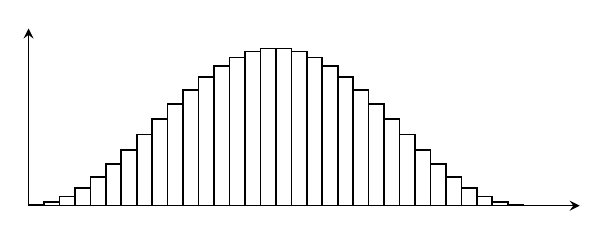
\begin{tikzpicture}[>=stealth, scale=2, semithick]
        \draw[->] (0, 0) -- (0, 1.125);
        \draw[->] (0, 0) -- (3.5, 0);
        \foreach \t in {0, 1, ..., 31} {
            \draw (pi * \t / 32, 0) rectangle ({pi * (\t + 1) / 32}, {16 * 2 / 32 * sin(180 / pi * pi * (\t + 0.5) / 32)^2});
        };
    \end{tikzpicture}
    \caption{Sketch of the amplitudes, here for \(t = 5\) and scaled by \(16\).}
    \label{sketch_of_the_amplitudes}
\end{figure}

\begin{figure}[!hbtp]
    \centering
    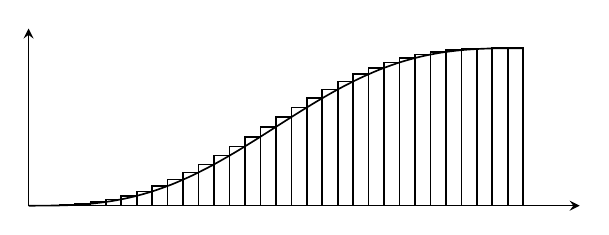
\begin{tikzpicture}[>=stealth, scale=2, semithick]
        \draw[->] (0, 0) -- (0, 1.125);
        \draw[->] (0, 0) -- (3.5, 0);
        \xdef\area{0};
        \foreach \t in {0, 1, ..., 31} {
            \pgfmathparse{\area + 2 / 32 * sin(180 / pi * pi * (\t + 0.5) / 32)^2};
            \xdef\area{\pgfmathresult};
            \draw (pi * \t / 32, 0) rectangle ({pi * (\t + 1) / 32}, {\area});
        };
        \draw[domain=0:3.1416, smooth] plot ({\x},  {1/32*(32/pi*\x-sin(deg(2*\x))/(2*sin(deg(pi/32))))});
    \end{tikzpicture}
    \caption{Sketch of the cumulative amplitude sums, here for \(t = 5\) and scaled by \(1\). The associated integral function of the probability distribution \(p\), \(P\), as found in the proof of \Cref{hhl_clock_initialization}, is also depicted.}
    \label{sketch_of_the_cumulative_amplitude_sums}
\end{figure}

As for the procedure \(\mathcal{B}\): We have discussed the problem of quantum state generation in \Cref{quantum_state_generation_based_on_efficiently_integrable_probability_distributions}. Efficient state generation is a key issue here, as an inefficient state generation procedure will drown the runtime of the HHL algorithm, as can be seen in \Cref{hhl_algorithm}.

\subsection{Analysis for Well-Conditioned Matrices \draftcommentgreen{DONE}}

We present the analysis from \cite{Harrow2008} with slightly different constants in the results. We assume, that none of the subprocedures produce an error, which one may consider to be a reasonable assumption due to our previous discussion on the complexity for keeping a low error gap for each subprocedure. Consider again the assumptions made in \Cref{hhl_problem_description_and_assumptions}.

\paragraph*{First Steps} \phantom{}\\\phantom{}

We first follow along the description of the algorithm in \Cref{hhl_algorithm} and observe the change of the registers. Initializing the first two registers yields
\begin{align}
    \ket{0}\ket{0}\ket{0} \xmapsto{\mathcal{T} \otimes \mathcal{B} \otimes E_3} \sqrt{\frac{2}{T}} \sum_{\tau = 0}^{T-1} \sin\left(\frac{\pi(\tau+\frac{1}{2})}{T}\right)\ket{\tau} \ket{b} \ket{0} = \sqrt{\frac{2}{T}} \sum_{j = 1}^N \beta_j \sum_{\tau = 0}^{T-1} \sin\left(\frac{\pi(\tau+\frac{1}{2})}{T}\right)\ket{\tau} \ket{v_j} \ket{0}
\end{align}
After that, applying \(\che_{T, N, A, t_0} \otimes E_3\) with effect on the first two registers and the use of \Cref{exponential_eigenvalue_theorem} gives
\begin{align}
    &\sqrt{\frac{2}{T}} \sum_{j = 1}^N \beta_j \sum_{\tau = 0}^{T-1} \sin\left(\frac{\pi(\tau+\frac{1}{2})}{T}\right)\che_{T, N, A, t_0} \ket{\tau} \ket{v_j} \ket{0}\\
    =& \sqrt{\frac{2}{T}} \sum_{j = 1}^N \beta_j \sum_{\tau = 0}^{T-1} \sin\left(\frac{\pi(\tau+\frac{1}{2})}{T}\right) e^{i \lambda_j \tau t_0 / T} \ket{\tau} \ket{v_j} \ket{0}
\end{align}
Now we apply \(\qft^\dagger_T \otimes E_{N \cdot 3}\), which, after some reordering, results in
\begin{align}
    &\sqrt{\frac{2}{T}} \sum_{j = 1}^N \beta_j \sum_{\tau = 0}^{T-1} \sin\left(\frac{\pi(\tau+\frac{1}{2})}{T}\right) e^{i \lambda_j \tau t_0 / T} \qft^\dagger_T \ket{\tau} \ket{v_j} \ket{0}\\
    =& \frac{\sqrt{2}}{T} \sum_{j = 1}^N \beta_j \sum_{\tau = 0}^{T-1} \sin\left(\frac{\pi(\tau+\frac{1}{2})}{T}\right) e^{i \lambda_j \tau t_0 / T} \sum_{k=0}^{T-1} e^{-2 \pi i k \tau / T} \ket{k} \ket{v_j} \ket{0}\\
    =& \frac{\sqrt{2}}{T} \sum_{j = 1}^N \beta_j \sum_{k = 0}^{T-1} \left(\sum_{\tau = 0}^{T-1} \sin\left(\frac{\pi(\tau+\frac{1}{2})}{T}\right) e^{\frac{i \tau}{T} (\lambda_j t_0 - 2 \pi k)}\right) \ket{k} \ket{v_j} \ket{0}\\
    \overset{\ref{hhl_first_steps_calc_1}}{=}& \sum_{j = 1}^N \beta_j \sum_{k = 0}^{T-1} \ajk \ket{k} \ket{v_j} \ket{0}
\end{align}

\begin{enumerate}[label=(\arabic*)]
    \item \label{hhl_first_steps_calc_1} Note that we define for these indices \(j, k\) the values \(\ajk \in \mathbb{C}\) and \(\djk \in \mathbb{R}\) via
    \begin{align}
        \ajk \coloneqq \frac{\sqrt{2}}{T} \sum_{\tau = 0}^{T-1} \sin\left(\frac{\pi(\tau+\frac{1}{2})}{T}\right) e^{\frac{i \tau}{T} \djk} \qquad \djk \coloneqq \lambda_j t_0 - 2 \pi k \label{ajk_djk_helpers}
    \end{align}
\end{enumerate}

This intermediate result corresponds to a ''good'' approximation of the eigenvalues of \(A\), as we will prove in the following paragraph. We only make one small observation.

\begin{observation} \label{basic_alpha_bound_and_alphas_are_prob_distr}
    We have \(\sum_{k=0}^{T-1} |\ajk|^2 = 1\). This follows by considering \(\ket{b} = \ket{v_j}\) and thus having
    \begin{align}
        \sum_{j=1}^N \beta_j \sum_{k=0}^{T-1} \ajk \ket{k}\ket{v_j}\ket{0} = \sum_{k=0}^{T-1} \ajk \ket{k}\ket{v_j}\ket{0}
    \end{align}
    be a valid quantum state with the \(\ajk\) values being independent of \(\beta_j\). Furthermore, we have \(|\ajk| \leq 1\).
\end{observation}

\begin{figure}[!hbtp]
    \centering
    \begin{tikzpicture}[>=stealth, semithick]
        \newcommand{\dx}{2.5}
        \node[below] at (0*\dx, 0) {\(0\)};
        \node[below] at (1*\dx, 0) {\(2\pi\)};
        \draw (0*\dx, 0) -- (1*\dx, 0);
        \foreach \x in {0, 1, ..., 5}{
            \draw[shift={(\x*\dx, 0)}] (0, -2pt) -- (0, 2pt);
        };
        \node (0) at (1.5*\dx, 0) {...};
        \node (01) at (1.5*\dx, 0.25cm) {...};
        \node (02) at (1.5*\dx, 0.5cm) {...};
        \draw (1*\dx, 0) -- (0);
        \draw (0) -- (2*\dx, 0);
        \node[below] at (2*\dx, 0) {\(2\pi(k-1)\)};
        \node[below] at (3*\dx, 0) {\(2\pi k\)};
        \draw (2*\dx, 0) -- (3*\dx, 0);
        \node (1) at (3.5*\dx, 0) {...};
        \node (11) at (3.5*\dx, 0.25cm) {...};
        \node (12) at (3.5*\dx, 0.5cm) {...};
        \draw (3*\dx, 0) -- (1);
        \draw (1) -- (4*\dx, 0);
        \node[below] at (4*\dx, 0) {\(2\pi(T-2)\)};
        \node[below] at (5*\dx, 0) {\(2\pi(T-1)\)};
        \draw (4*\dx, 0) -- (5*\dx, 0);
        \draw[shift={(2.7*\dx, 0)}] (0, -2pt) -- (0, 2pt);
        \node[below] at (2.7*\dx, 0) {\(\lambda_j t_0\)};
        \draw[|-] (0*\dx, 0.25cm) -- (01) node[left, pos=0] {\(|\delta_{j, 0}|\)};
        \draw[-|] (01) -- (2.7*\dx, 0.25cm);
        \draw[|-] (1*\dx, 0.5cm) -- (02) node[left, pos=0] {\(|\delta_{j, 1}|\)};
        \draw[-|] (02) -- (2.7*\dx, 0.5cm);
        \draw[|-|] (2*\dx, 0.75cm) -- (2.7*\dx, 0.75cm) node[left, pos=0] {\(|\delta_{j, k-1}|\)};
        \draw[|-] (2.7*\dx, 0.25cm) -- (11);
        \draw[-|] (11) -- (5*\dx, 0.25cm) node[right] {\(|\delta_{j, T-1}|\)};
        \draw[|-] (2.7*\dx, 0.5cm) -- (12);
        \draw[-|] (12) -- (4*\dx, 0.5cm) node[right] {\(|\delta_{j, T-2}|\)};
        \draw[|-|] (2.7*\dx, 0.75cm) -- (3*\dx, 0.75cm) node[right, pos=1] {\(|\delta_{j, k}|\)};
    \end{tikzpicture}
    \caption{A line representing \([0, 2 \pi (T-1)]\) with marks for understanding the behavior of the approximations for one \(\djk\) value. We assume an appropriate choice for \(t\), as described in this text. In this case, the approximation seems to be of poor quality, increasing \(t\) will improve the accuracy as then the interval \([2\pi(k-1), 2\pi k]\) will be split in half and \(2\pi(2k-1)\) will give a better approximation.}
    \label{delta_values_visualized}
\end{figure}

\paragraph*{Analysis of the Phase Estimation} \label{hhl_phase_estimation_analysis} \phantom{}\\\phantom{}

The following analysis of the coefficients \(\ajk\) is based on the original HHL paper \cite[pp. 10-11]{Harrow2008} and Dervovic et al. \cite[pp. 32-33]{Dervovic2018}, but we do not fully agree with the assumptions used. Our goal is to prove, that for each \(j \in [1, N]_{\mathbb{N}}\), there are at most two values \(k \in [0, T-1]_{\mathbb{N}}\), where the coefficients \(\ajk\) concentrate at, meaning that the sum of their squared magnitudes is large in comparison to the magnitude sums of the exponentially many other approximations, and, such that \(2 \pi k / t_0\) is a good approximation of \(\lambda_j\). To get some intuition on this analysis, notice, that the value \(\djk\) becomes very small if \(2 \pi k / t_0 \approx \lambda_j\). We try to carry this intuition over to the coefficients \(\ajk\). The main result of this paragraph will be the following theorem.

\begin{theorem} \label{alphas_yield_good_approximation}
    For the HHL phase estimation of an eigenvalue \(\lambda_j\) with \(j \in [1, N]_{\mathbb{N}}\) arbitrary, but fixed, it holds, that
    \begin{align}
        \sum_{\substack{k \in [0, T-1]_{\mathbb{N}}\\|\djk| \geq 2\pi}} |\ajk|^2 < \frac{7}{10}
    \end{align}
\end{theorem}

Let \(j\), \(k\) as in \Cref{ajk_djk_helpers} be arbitrary, but fixed with \(|\djk| \geq 2\pi\).

\begin{observation} \label{inner_amplitude_bounds}
    By definition and \(\lambda_j \in \left[\frac{1}{\kappa}, 1\right]\), we have \(|\djk| \leq \max(\{t_0, 2 \pi (T-1)\})\). Since, due to the algorithm description, we assume a choice of \(t\), s.t. \(t_0 \leq 2 \pi (T-1)\), as \(T \geq t_0/2\pi+1\), we get
    \[
        2\pi \leq |\djk| \leq 2 \pi (T-1)
    \]
\end{observation}

We disagree with the assumption by the HHL authors, that \(|\delta_{i, j}| \leq T/10\) \cite[p. 11]{Harrow2008}. If one applies the algorithm on any unit matrix and chooses \(t_0\) to be incredibly high, whilst using only few helper qubits, the bound will not hold. In the following, we present a detailled derivation of the alternative representation of the \(\ajk\) values, which can be found in \cite[p. 11]{Harrow2008}.

\begin{restatable}{lemma}{sinebound} \label{sine_bound}
    The following bounds hold for any \(x \in \mathbb{R}_{\geq 0}\):
    \begin{align}
        x - \frac{x^3}{6} \leq \sin(x) \leq x
    \end{align}
    With strict inequalities for \(x \neq 0\).
\end{restatable}

The lower bound is not obvious. We present the proof of this rather elementary bound in \Cref{sine_bound_proof}.

\begin{lemma} \label{alpha_values_rewrite}
    The following statements hold.
    \begin{enumerate}[label=(\roman*)]
        \item[\ref{alpha_values_rewrite_1}] For \(\djk \notin \{\pm \pi\}\), it holds, that
        \begin{align}
            \ajk = -e^{i\frac{\djk}{2}\left(1-\frac{1}{T}\right)}\frac{\sqrt{2}\cos\left(\frac{\djk}{2}\right)}{T} \frac{\cos\left(\frac{\djk}{2T}\right)\sin\left(\frac{\pi}{2T}\right)}{\sin\left(\frac{\djk+\pi}{2T}\right)\sin\left(\frac{\djk-\pi}{2T}\right)}
        \end{align}
        \item[\ref{alpha_values_rewrite_2}] The function
        \begin{align}
            \xi \colon (-2\pi, 2\pi) \setminus \{\pm \pi\} \to \mathbb{R}, \delta \mapsto \frac{2}{T^2} \sin^2\left(\frac{\pi}{2T}\right) \frac{\cos^2\left(\frac{\delta}{2}\right)\cos^2\left(\frac{\delta}{2T}\right)}{\sin^2\left(\frac{\delta+\pi}{2T}\right)\sin^2\left(\frac{\delta-\pi}{2T}\right)}
        \end{align}
        can be continuously extended to \((-2\pi, 2\pi)\).
    \end{enumerate}
\end{lemma}

\begin{proof}
    \begin{enumerate}[label=(\roman*)]
        \item \label{alpha_values_rewrite_1} We give thorough explanations to the following large computation.
        \begin{align}
            \ajk &= \frac{\sqrt{2}}{T} \sum_{\tau = 0}^{T-1} \sin\left(\frac{\pi(\tau+\frac{1}{2})}{T}\right) \exp\left(\frac{i \tau}{T} \djk\right)\\
            &\overset{\ref{alpha_values_rewrite_step_1}}{=} \frac{1}{i\sqrt{2}T} \sum_{\tau = 0}^{T-1} \exp\left(\frac{i\tau}{T}\djk\right)\left(\exp\left(i\frac{\pi(\tau+\frac{1}{2})}{T}\right)-\exp\left(-i\frac{\pi(\tau+\frac{1}{2})}{T}\right)\right)\\
            &\overset{\ref{alpha_values_rewrite_step_2}}{=} \frac{1}{i\sqrt{2}T} \left(\exp\left(\frac{i\pi}{2T}\right)\sum_{\tau = 0}^{T-1}\exp\left(i\tau\frac{\djk+\pi}{T}\right) - \exp\left(-\frac{i\pi}{2T}\right)\sum_{\tau = 0}^{T-1}\exp\left(i\tau\frac{\djk-\pi}{T}\right)\right)\\
            &\overset{\ref{alpha_values_rewrite_step_3}}{=} \frac{1}{i\sqrt{2}T} \left(\exp\left(\frac{i\pi}{2T}\right)\frac{1-e^{i(\djk+\pi)}}{1-e^{i\frac{\djk+\pi}{T}}} - \exp\left(-\frac{i\pi}{2T}\right)\frac{1-e^{i(\djk-\pi)}}{1-e^{i\frac{\djk-\pi}{T}}}\right) \label{special_djk_bounds}\\
            &\overset{\ref{alpha_values_rewrite_step_4}}{=} \frac{1+e^{i\djk}}{i\sqrt{2}T} \left(\frac{e^{-i\frac{\djk}{2T}}}{e^{-i\frac{\djk+\pi}{2T}}-e^{i\frac{\djk+\pi}{2T}}} - \frac{e^{-i\frac{\djk}{2T}}}{e^{-i\frac{\djk-\pi}{2T}}-e^{i\frac{\djk-\pi}{2T}}}\right)\\
            &\overset{\ref{alpha_values_rewrite_step_5}}{=} \frac{(1+e^{i\djk})e^{-i\frac{\djk}{2T}}}{i\sqrt{2}T} \left(\frac{1}{-2i\sin\left(\frac{\djk+\pi}{2T}\right)} - \frac{1}{-2i\sin\left(\frac{\djk-\pi}{2T}\right)}\right)\\
            &\overset{\ref{alpha_values_rewrite_step_6}}{=} e^{i\frac{\djk}{2}\left(1-\frac{1}{T}\right)}\frac{\cos\left(\frac{\djk}{2}\right)}{\sqrt{2}T} \frac{\sin\left(\frac{\djk-\pi}{2T}\right)-\sin\left(\frac{\djk+\pi}{2T}\right)}{\sin\left(\frac{\djk+\pi}{2T}\right)\sin\left(\frac{\djk-\pi}{2T}\right)}\\
            &\overset{\ref{alpha_values_rewrite_step_7}}{=} -e^{i\frac{\djk}{2}\left(1-\frac{1}{T}\right)}\frac{\sqrt{2}\cos\left(\frac{\djk}{2}\right)}{T} \frac{\cos\left(\frac{\djk}{2T}\right)\sin\left(\frac{\pi}{2T}\right)}{\sin\left(\frac{\djk+\pi}{2T}\right)\sin\left(\frac{\djk-\pi}{2T}\right)}
        \end{align}
    
        \begin{enumerate}[label=(\arabic*), wide]
            \item \label{alpha_values_rewrite_step_1} Use the definition of the sine with the complex exponential function, see \Cref{exponential_sine_and_cosine}.
            \item \label{alpha_values_rewrite_step_2} Reorder the terms wrt. the dependency on \(\tau\).
            \item \label{alpha_values_rewrite_step_3} Use the geometric sum. With \(\djk \notin \{\pm \pi\}\), it is assured, that we do not add up ones, as otherwise the geometric sum does not apply here in this form.
            \item \label{alpha_values_rewrite_step_4} Notice \(e^{i(\djk+\pi)} = -e^{i\djk} = e^{i(\djk-\pi)}\) by definition. Thus, we first factor out \(1+e^{i\djk}\). Expand the terms by \(e^{-i\frac{\djk+\pi}{2T}}\) and \(e^{-i\frac{\djk-\pi}{2T}}\), through which the factors \(e^{\frac{i\pi}{2T}}\) and \(e^{-\frac{i\pi}{2T}}\) get cancelled out.
            \item \label{alpha_values_rewrite_step_5} Factor out the numerators and use the definition of the sine via the complex exponential function, see \Cref{exponential_sine_and_cosine}, in the denominators.
            \item \label{alpha_values_rewrite_step_6} Factoring out \(1/(-2i)\) from the sums yields a denominator of \(2\sqrt{2}T\). Now, using the exponential form of the \emph{cosine} function for once, we also obtain:
            \begin{align}
                (1+e^{i\djk})e^{-i\frac{\djk}{2T}} = (e^{-i\frac{\djk}{2}}+e^{i\frac{\djk}{2}})e^{i\frac{\djk}{2}\left(1-\frac{1}{T}\right)} = 2\cos\left(\frac{\djk}{2}\right)e^{i\frac{\djk}{2}\left(1-\frac{1}{T}\right)}
            \end{align}
            At last, we expand the right terms. This fixes one calculation mistake of the original paper: The \(\sqrt{2}\) is part of the denominator.
            \item \label{alpha_values_rewrite_step_7} We use the sine addition theorem, see \Cref{sine_and_cosine_addition_theorem}. With the asymmetry of the sine function, and the symmetry of the cosine function, this yields:
            \begin{align}
                \sin\left(\frac{\djk-\pi}{2T}\right)-\sin\left(\frac{\djk+\pi}{2T}\right) &= \cos\left(\frac{\djk}{2T}\right)\sin\left(\frac{-\pi}{2T}\right)-\cos\left(\frac{\djk}{2T}\right)\sin\left(\frac{\pi}{2T}\right)\\
                &= -2\cos\left(\frac{\djk}{2T}\right)\sin\left(\frac{\pi}{2T}\right)
            \end{align}
        \end{enumerate}
        \item \label{alpha_values_rewrite_2} Notice \(\xi(-\delta) = \xi(\delta)\) due to \(\sin^2\left(\frac{-\delta+\pi}{2T}\right)\sin^2\left(\frac{-\delta-\pi}{2T}\right) = \sin^2\left(\frac{\delta+\pi}{2T}\right)\sin^2\left(\frac{\delta-\pi}{2T}\right)\) and the axial symmetry of the cosine. It thus suffices to prove the existence of \(\lim_{\delta \to \pi} \xi(\delta)\). We have
        \begin{align}
            \lim_{\delta \to \pi} \frac{\cos\left(\frac{\delta}{2}\right)\cos\left(\frac{\delta}{2T}\right)}{\sin\left(\frac{\delta+\pi}{2T}\right)\sin\left(\frac{\delta-\pi}{2T}\right)} = \frac{\evalat{\frac{\partial}{\partial \delta} \cos\left(\frac{\delta}{2}\right)\cos\left(\frac{\delta}{2T}\right)}{\pi}}{\frac{1}{2T}\sin\left(\frac{\pi}{T}\right)}
        \end{align}
        using the rule of Bernoulli-L'Hospital \cite[pp. 150-151]{Koenigsberger2003} and
        \begin{align}
            \frac{\partial}{\partial \delta} \sin\left(\frac{\delta+\pi}{2T}\right)\sin\left(\frac{\delta-\pi}{2T}\right) &= \frac{1}{2T}\left(\cos\left(\frac{\delta+\pi}{2T}\right)\sin\left(\frac{\delta-\pi}{2T}\right)+\sin\left(\frac{\delta+\pi}{2T}\right)\cos\left(\frac{\delta-\pi}{2T}\right)\right)\\
            &= \frac{1}{2T}\sin\left(\frac{\delta}{T}\right)
        \end{align}
        using the product rule of differential calculus and \Cref{sine_and_cosine_addition_theorem}. Taking the continuity of \(\delta \mapsto \delta^2\) into account, we obtain the statement.
    \end{enumerate}

    This concludes the proof.
\end{proof}

Part \ref{alpha_values_rewrite_2} of this lemma will not be used, its importance lies in the fact, that the \(\ajk\) values do not ''blow up'' for values \(|\djk|\) near \(\pi\). We now present a descriptive analytic proof for the bound concentration, i.e., that for \(j\) and \(k\) with \(|\djk| < 2\pi\), we have a good approximation of \(\lambda_j\) by \(\frac{2 \pi k}{t_0}\). It holds, that
\begin{align}
    |\ajk| \overset{\ref{small_ajk_calc_1}}{=} \frac{\sqrt{2}\left|\cos\left(\frac{\djk}{2}\right)\right|}{T} \frac{\left|\cos\left(\frac{\djk}{2T}\right)\right|\sin\left(\frac{\pi}{2T}\right)}{\sin\left(\frac{\djk+\pi}{2T}\right)\sin\left(\frac{\djk-\pi}{2T}\right)} \overset{\ref{small_ajk_calc_2}}{<} \frac{\pi}{\sqrt{2}T^2} \frac{1}{\sin\left(\frac{\djk+\pi}{2T}\right)\sin\left(\frac{\djk-\pi}{2T}\right)} \label{first_alpha_magnitude_rewrite}
\end{align}
\begin{enumerate}[label=(\arabic*), wide]
    \item \label{small_ajk_calc_1} Taking the complex magnitude respects products, \(\left|-\exp(i\frac{\djk}{2}\left(1-\frac{1}{T}\right))\right| = 1\) and  \(\frac{\pi}{2T} \in \left(0, \frac{\pi}{64}\right)\), where the sine is positive. Furthermore, for \(\djk > 0\), we have \(\frac{\djk+\pi}{2T}, \frac{\djk-\pi}{2T} \in \left[\frac{\pi}{2T}, \pi - \frac{\pi}{2T}\right]\), where the sine is also positive. We also have \(\sin\left(\frac{-\djk+\pi}{2T}\right)\sin\left(\frac{-\djk-\pi}{2T}\right) = \sin\left(\frac{\djk-\pi}{2T}\right)\sin\left(\frac{\djk+\pi}{2T}\right)\), so we can leave out taking the magnitude again.
    \item \label{small_ajk_calc_2} Since \(|\cos| \leq 1\) with strict inequality for arguments outside of \(\pi \mathbb{Z}\), and \Cref{sine_bound}.
\end{enumerate}

We want to further study the result analytically.

\begin{lemma} \label{continuous_delta_alpha_behavior}
    Define the auxiliary function
    \begin{align}
        h\colon \mathbb{R} \setminus \{2 \pi k T \pm \pi \mid k \in \mathbb{Z}\} \to \mathbb{R}_{> 0}, \delta \mapsto \frac{\pi}{\sqrt{2}T^2} \frac{1}{\sin\left(\frac{\delta+\pi}{2T}\right)\sin\left(\frac{\delta-\pi}{2T}\right)}
    \end{align}
    and let \(h^\pm \coloneqq h|_{[\pm2\pi(T-1), \pm2\pi] \cup [\pm2\pi, \pm2\pi(T-1)]}\) each yielding \(h^+\) and \(h^-\). We have
    \begin{enumerate}[label=(\roman*)]
        \item \(h^-(-\delta) = h^+(\delta)\) for \(\delta \in [2\pi, 2\pi(T-1)]\).
        \item \(h^+\) is symmetric wrt. \(\pi T\).
        \item \(h^+|_{[2\pi, \pi T]}\) strictly descends.
    \end{enumerate}
\end{lemma}

\begin{proof}
    \begin{enumerate}[label=(\roman*)]
        \item We have proven this in \ref{small_ajk_calc_1} for \Cref{first_alpha_magnitude_rewrite}.
        \item If \(\delta \in [2\pi, \pi T]\), then \(2 \pi T - \delta \in [\pi T, 2\pi(T-1)]\). Especially
        \begin{align}
            \sin\left(\frac{(2 \pi T - \delta) + \pi}{2T}\right)\sin\left(\frac{(2 \pi T - \delta) - \pi}{2T}\right) &= \sin\left(\pi - \frac{\delta - \pi}{2T}\right)\sin\left(\pi - \frac{\delta + \pi}{2T}\right)\\
            &= \sin\left(\frac{\delta - \pi}{2T}\right)\sin\left(\frac{\delta + \pi}{2T}\right)
        \end{align}
        \item As \(\frac{\partial}{\partial \delta} \sin\left(\frac{\delta+\pi}{2T}\right)\sin\left(\frac{\delta-\pi}{2T}\right) = \frac{1}{2T} \sin\left(\frac{\delta}{T}\right) \geq 0\) in \([2\pi, \pi T]\), see \Cref{l_functions_derivatives_1}, the function stricly descends. Note, that the right bound does not matter by the definition of strict monotonicity.
    \end{enumerate}
\end{proof}

\begin{remark}
    The consequence of this lemma is, that we can reduce the calculation of \(h\) for any \(\djk\) by mirroring the value at most twice, once around \(x = 0\) and once around \(x = \pi T\). As the \(\djk\) values are evenly spread on an interval of length \(2\pi (T-2)\), we can further bound any sum over all \(\ajk\) values by only considering the values of \(h\) in \([2\pi, \pi (T-1)]\). We shall use this thought in the proof of \Cref{alphas_yield_good_approximation}.
\end{remark}

\begin{restatable}{lemma}{sinecomplemma} \label{sine_comp_lemma}
    Defining for \(T \coloneqq 2^t\), \(t \in \mathbb{N}_{\geq 5}\)
    \begin{align}
        l^\uparrow\colon [2\pi, \pi T] \to \mathbb{R}, \delta \mapsto \sin\left(\frac{\delta + \pi}{2T}\right)\sin\left(\frac{\delta - \pi}{2T}\right) \qquad l^\downarrow\colon [2\pi, \pi T] \to \mathbb{R}, \delta \mapsto \frac{c_1}{\pi^2} \frac{\delta^2}{T^2}
    \end{align}
    where \(c_1 \coloneqq 0.9975 < \sin\left(\frac{\pi}{2}-\frac{\pi}{64}\right)\), we have \(l^\uparrow > l^\downarrow\).
\end{restatable}

We leave out the technicalities of this lemma and prove it in the appendix, see \Cref{sine_comp_lemma_proof}. Consider the illustration with a summary of the argument in \Cref{sine_comp_lemma_visualized}.

\begin{figure}[!hbtp]
    \centering
    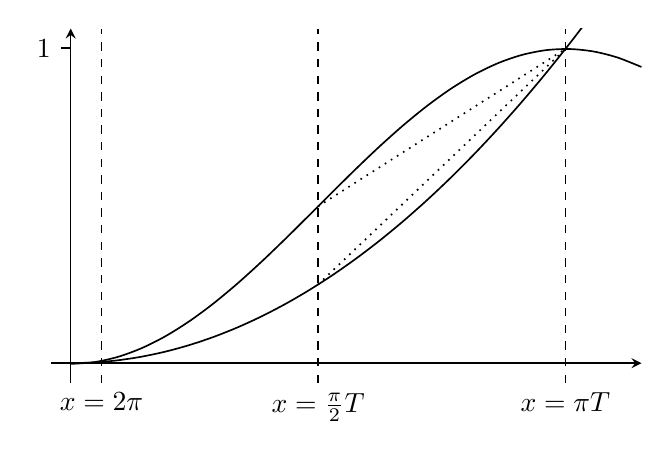
\begin{tikzpicture}[>=stealth, scale=2, semithick]
        \draw[->] (-0.125, 0) -- (3.625, 0);
        \draw[->] (0, -0.125) -- (0, 2.125);

        \draw (-0.0625, 2) -- (0, 2) node[left, pos=0] {\(1\)};
        \draw[dashed] (0.1963, -0.125) -- (0.1963, 2.125) node[below, pos=0] {\(x = 2\pi\)};
        \draw[dashed] (1.5710, -0.125) -- (1.5710, 2.125) node[below, pos=0] {\(x = \frac{\pi}{2}T\)};
        \draw[dashed] (3.1416, -0.125) -- (3.1416, 2.125) node[below, pos=0] {\(x = \pi T\)};

        \clip (-0.125, -0.125) rectangle (3.625, 2.125);
        \draw[domain=0:3.625, range=0:2, smooth] plot ({\x},  {2 * sin(deg((\x*32+pi)/64)) * sin(deg((\x*32-pi)/64))});
        \draw[domain=0:3.625, range=0:2, smooth] plot ({\x},  {2 * 0.9975/(pi^2) * (\x^2*32^2)/(32^2)});
        \draw[dotted] (1.5710, 2 * 0.4976) -- (3.1416, 2 * 0.9976);
        \draw[dotted] (1.5710, 2 * 0.2494) -- (3.1416, 2 * 0.9975);
    \end{tikzpicture}
    \caption{Graph of \(l^\uparrow\) and \(l^\downarrow\) für \(t = 5\). The \(x\)-axis is scaled by \(1/T\), the \(y\)-axis is scaled by \(2\) and the entire plot is scaled by 2. The vertical lines \(x = 2\pi\), \(x = \frac{\pi}{2} T\) and \(x = \pi T\) are marked. In the interval \([2\pi, \pi T/2]\), \(l^\uparrow\) grows faster than \(l^\downarrow\), while being larger at the interval boundaries. In \([\pi T / 2, \pi T]\), \(l^\uparrow\) is convex, and larger at the boundary points, while \(l^\downarrow\) is concave. The convexity and concavity argument is illustrated by the dotted lines. These facts conclude \(l^\uparrow > l^\downarrow\). The rigorous formulation can be found in the appendix, as said.}
    \label{sine_comp_lemma_visualized}
\end{figure}

\begin{lemma} \label{alpha_delta_values_relation}
    For \(2\pi \leq \djk \leq \pi T\), we have
    \begin{align}
        |\ajk| < \frac{22}{\djk^2}
    \end{align}
\end{lemma}

\begin{proof}
    \Cref{sine_comp_lemma} and \Cref{alpha_values_rewrite} directly give us
    \begin{align}
        |\ajk| < \frac{\pi}{\sqrt{2}T^2} \frac{\pi^2}{c_1} \frac{T^2}{\djk^2} < \frac{22}{\djk^2}
    \end{align}
\end{proof}

\begin{remark}
    For a guarantee of a good approximation of the eigenvalues, \Cref{helper_qubits_needed} shows, that at least five qubits are needed.
\end{remark}

Now we are able to give the proof of the main theorem of this subsection.

\begin{proof}[Proof of \Cref{alphas_yield_good_approximation}]
    Due to the behavior of \(h\) in \Cref{continuous_delta_alpha_behavior}, we have
    \begin{align}
        \sum_{\substack{k \in [0, T-1]_{\mathbb{N}}\\|\djk| \geq 2\pi}} |\ajk|^2 \overset{\ref{continuous_delta_alpha_behavior_1}}{<} \sum_{k=1}^{T-1} h(2 \pi k)^2 \overset{\ref{continuous_delta_alpha_behavior_2}}{<} 2\sum_{k=1}^\infty \frac{22^2}{16\pi^4k^4} \overset{\ref{continuous_delta_alpha_behavior_3}}{=} 2 \cdot \frac{22^2}{16 \cdot 90} < \frac{7}{10}
    \end{align}
    \begin{enumerate}[label=(\arabic*), wide]
        \item \label{continuous_delta_alpha_behavior_1} The values \(\djk\) are positioned in distance \(2\pi\) to each closest neighbor. Consider for each \(k\), that \(|\djk| \in [2 \pi k', 2 \pi (k'+1)]\) for some \(k' \in \mathbb{Z}\). With the monotonicity behavior of \(h\), as in \Cref{continuous_delta_alpha_behavior}, we thus have the upper bound using \(h^2\) at either \(2 \pi k'\) or \(2 \pi (k'+1)\) for this value \(|\ajk|^2\). To observe the statement for the sum, consider for a \(k\) with \(\djk < 0\), that mirroring, i.e. taking \(h^2(-\djk)\) for the strict upper bound, and then mirroring at \(\pi T\), gives the upper bound, and that no other element is then contained in the associated \(2 \pi\)-sized interval, in which \(2 \pi T + \djk\) lies, as then we have \(\delta_{j, 0} - \delta_{j, T-1} > 2 \pi (T-1)\), which is a contradiction to the definition of the \(\djk\) values.
        \item \label{continuous_delta_alpha_behavior_2} Following our previous considerations, we upper bound the values for \(\djk \in [2\pi, \pi T]\) twice and let them tend to infinity for a constant upper bound.
        \item \label{continuous_delta_alpha_behavior_3} Using \Cref{zeta_two}.
    \end{enumerate}
\end{proof}

\begin{remark} \label{eigenvalue_approximations_notation}
    With the last theorem proven, we will now use the notation \(\ket*{\tlk} \coloneqq \ket{k}\), \(k \in [0, T-1]_{\mathbb{N}}\), following \cite[p. 6]{Harrow2008}, for the basis states, where \(\tlk \coloneqq \frac{2 \pi k}{t_0}\). Note that with this notation, we indicate that for some such \(k\), \(\tlk\) gives a good approximation for some eigenvalue \(\lambda_j\), \(j \in [1, N]_{\mathbb{N}}\).
\end{remark}

The following theorem further elaborates the existence of a close approximation.

\begin{theorem}[Existence of Eigenvalue Approximations] \label{existence_of_eigenvalue_approximations}
    The following statements hold for any fixed \(j \in [1, N]_{\mathbb{N}}\).
    \begin{enumerate}[label=(\roman*)]
        \item[\ref{existence_of_eigenvalue_approximations_1}] There is a \(k \in [0, T-1]_{\mathbb{N}}\) with \(|\djk| < 2\pi\).
        \item[\ref{existence_of_eigenvalue_approximations_2}] For every \(k \in [0, T-1]_{\mathbb{N}}\) with \(|\djk| < 2\pi\), we have
        \begin{align}
            |\tlk - \lambda_j| < \frac{1}{4\kappa}
        \end{align}
        and thus
        \begin{align}
            \tlk \in \left(\frac{3}{4\kappa}, 1 + \frac{1}{4\kappa}\right)
        \end{align}
    \end{enumerate}
\end{theorem}

\begin{proof} We prove the statements in series.

    \begin{enumerate}[label=(\roman*)]
        \item \label{existence_of_eigenvalue_approximations_1} Fix \(j\) and consider under the condition \(\djk \leq 0\)
        \begin{align}
            0 \leq -\djk = 2 \pi k - \lambda_jt_0 < 2\pi \leadsto \frac{\lambda_jt_0}{2\pi} < k < \frac{\lambda_jt_0}{2\pi}+1
        \end{align}
        as \(\frac{\lambda_jt_0}{2\pi} \in (0, T-1)\), we may thus choose \(k \coloneqq \left\lfloor \frac{\lambda_jt_0}{2\pi} \right\rfloor\) or \(k = 1\) for \(\frac{\lambda_jt_0}{2\pi} < 1\).
        \item \label{existence_of_eigenvalue_approximations_2}
        From the assumption and the definition of \(\djk\), we directly have
        \begin{align}
            |\lambda_j - \tlk| = \frac{|\djk|}{t_0} < \frac{2\pi}{t_0} = \frac{\pi\varepsilon}{100\kappa} \in \left(0, \frac{1}{4\kappa}\right)
        \end{align}
        The second statement follows directly.
    \end{enumerate}
     
\end{proof}

This proof is the main reason for our choice of \(\varepsilon\). In the second next subsection, we will also see the reason for our choice of \(t_0\).

\paragraph*{Inversion of the Eigenvalue Approximations} \label{hhl_inversion_of_approx} \phantom{} \vspace{\baselineskip}

With the eigenvalue approximations stored, we want to transfer them over into the amplitudes to obtain a form as in \Cref{corollary_inverse_spectral_decomposition}. The goal, as in \Cref{hhl_target_state}, is to obtain
\begin{align}
    \sum_{i=1}^N \frac{\beta_i}{\lambda_i} \ket{v_i}
\end{align}
in the input register. Rotating conditioned on a map of form \(\lambda \mapsto \arcsin\left(C/\lambda\right)\), where \(C \in (0, \lambda_{\min{}}(A)] \supseteq (0, \frac{1}{\kappa}]\) for normalization and \(\lambda_{\min{}}(A)\) as in \Cref{condition_number}, would suffice for this task, as we can verify by following along the calculations of the proof of \Cref{qutrit_rotation}. By measuring the helper qutrit and using amplitude amplification, we could obtain an approximation of the target state. The problem with this approach stems from the case, when the eigenvalues are incredibly small. Errors in the phase estimation, which can be quite large simply due large \(\djk\) values, see \Cref{delta_values_visualized}, and by a poorly chosen \(t_0\) value, can lead to poor result states. We need a more numerically stable procedure \cite[p. 33]{Dervovic2018}.

The HHL authors have their own procedure \(\mathcal{R}\), as mentioned in \Cref{hhl_algorithm}. The filter functions are piecewise continuous functions, induced by concatenations of the sine, cosine and inversion, as well as constant functions. Especially, in \(\left[\frac{1}{2\kappa}, \frac{1}{\kappa}\right)\), the sine and cosine functions have been concatenated with a linear transform, which transforms this interval into \(\left[0, \frac{\pi}{2}\right)\) isomorphically. This helps us understand the filter functions more: We want an approximately continuous function \(f\), that slowly descends for eigenvalues, which are not in the desired range, and a function \(g\), which becomes large for bad eigenvalues to fend off unacceptibly small eigenvalues. For an illustration, consider \Cref{filter_functions_visualization}. We further need a qutrit and this specific choice of the functions for a working analysis of the error.

\begin{figure}[!hbtp]
    \centering
    \begin{tikzpicture}[>=stealth, semithick]
        \draw[->] (0, -0.5) -- (0, 2.5);
        \draw[->] (-0.5, 0) -- (10.5, 0);
        \draw[-] (0, 2) -- (-0.05, 2) node[left] {\(\frac{1}{2}\)};
        \draw[-] (2, 0) -- (2, -0.05) node[below] {\(\frac{1}{2\kappa}\)};
        \draw[-] (4, 0) -- (4, -0.05) node[below] {\(\frac{1}{\kappa}\)};
        \draw (0, 2) -- (2, 2) node[above] {\(g\)};
        \draw[domain=4:10] plot ({\x}, {4*1/(2*10*\x/40)});
        \node[above] at (4, 2) {\(f\)};
        \draw[domain=2:4] plot ({\x}, {2*cos(90*(\x-2)/2)});
        \draw[domain=2:4] plot ({\x}, {2*sin(90*(\x-2)/2)});
    \end{tikzpicture}
    \caption{Sketch of the filter functions. Here an example for a matrix with eigenvalues \(1, 4, 7, 10\) and thus \(\kappa = 10\). The horizontal axis was scaled by \(20\), the vertical one by \(2\). One can very well see the rather sudden drop of \(g\) and the simultaneous entry of \(f\) in the interval \(\left[\frac{1}{2\kappa}, \frac{1}{\kappa}\right]\).}
    \label{filter_functions_visualization}
\end{figure}

The figure also demonstrates the effect of upper bounding \(\kappa\), which is that tinier eigenvalues are permitted for inversion. The qutrit rotation technique described in \Cref{qutrit_rotation} is also only applicable due to the following lemma.
\begin{lemma} \label{filter_functions_square_sum_bound}
    We have
    \begin{align}
        f^2 + g^2 \leq \frac{1}{4}
    \end{align}
    with equality in \(\left[0, \frac{1}{\kappa}\right]\).
\end{lemma}
\begin{proof}
    Following the definitions in \Cref{filter_functions}, in \(\left[0, \frac{1}{2\kappa}\right)\), \(f^2 + g^2 = \frac{1}{4}\), in \(\left[\frac{1}{2\kappa}, \frac{1}{\kappa}\right)\), we use \Cref{sine_and_cosine_addition_theorem} to have \(f^2 + g^2 = \frac{1}{4}\) and in \(\left[\frac{1}{\kappa}, \infty\right)\), \(f^2+g^2 \leq \frac{1}{4}\) with \(f^2\left(\frac{1}{\kappa}\right) = \frac{1}{4}\).
\end{proof}

By application of \(\mathcal{R}\), we obtain:
\begin{align}
    \sum_{j = 1}^N \beta_j \sum_{k = 0}^{T-1} \ajk \ket*{\tlk} \ket{v_j} \left(\sqrt{1-f^2(\tlk)-g^2(\tlk)}\ket{0}+f(\tlk)\ket{1}+g(\tlk)\ket{2}\right)
\end{align}
As in \Cref{hhl_algorithm_sketch}, we uncompute the first two registers. Keeping the concentration of the eigenvalue approximations in mind and following the calculations from before we gave the proof of \Cref{alphas_yield_good_approximation}, we apply \((\mathcal{T}^\dagger \otimes E_{N \cdot 3})(\che_{T, N, A, t_0}^\dagger \otimes E_3)(\qft_T \otimes E_{N \cdot 3})\) after making an approximation, giving
\begin{align}
    &\phantom{\approx} \sum_{j = 1}^N \beta_j \sum_{k = 0}^{T-1} \ajk \ket*{\tlk} \ket{v_j} \left(\sqrt{1-f^2(\tlk)-g^2(\tlk)}\ket{0}+f(\tlk)\ket{1}+g(\tlk)\ket{2}\right)\\
    &\approx \sum_{j = 1}^N \beta_j \sum_{k = 0}^{T-1} \ajk \ket*{\tlk} \ket{v_j} \left(\sqrt{1-f^2(\tlj)-g^2(\tlj)}\ket{0}+f(\tlj)\ket{1}+g(\tlj)\ket{2}\right)\\
    &\mapsto \sum_{j = 1}^N \beta_j \ket{0} \ket{v_j} \left(\sqrt{1-f^2(\tlj)-g^2(\tlj)}\ket{0}+f(\tlj)\ket{1}+g(\tlj)\ket{2}\right)
\end{align}
where \(\tlj\) denotes the best approximation of \(\lambda_j\) for each \(j\). Due to the possible entanglement of the ancilla qutrit with the clock register, we use \Cref{alphas_yield_good_approximation} to enable this approximation. We now apply amplitude amplification with the procedure so far and \(\chi\) as defined in \Cref{hhl_algorithm} to perform a measurement of a \(1\) in the ancilla qutrit. So for one measurement, assuming, that \(\tlj \in \left[\frac{1}{\kappa}, \infty\right)\) for all \(j \in [1, N]_{\mathbb{N}}\), we obtain the state
\begin{align}
    \frac{\sum_{j=1}^N \beta_j \frac{1}{2 \kappa \tlj} \ket{v_j}}{\sqrt{\sum_{j=1}^N |\beta_j|^2 \left|\frac{1}{2 \kappa \tlk}\right|^2}} \approx \frac{\sum_{j=1}^N \frac{\beta_j}{\lambda_j} \ket{v_j}}{\sqrt{\sum_{j=1}^N \left|\frac{\beta_j}{\lambda_j}\right|^2}} \text{ with probability } \sum_{j=1}^N |\beta_j|^2 \left|\frac{1}{2 \kappa \tlj}\right|^2
\end{align}
in the input register. We now make the latter parts of the argument precise.

\paragraph*{Choosing the Evolution Time} \phantom{}\\\phantom{}

For the phase estimation procedure to be successful, a well-chosen evolution time \(t_0\) is required. We follow along the error analysis of Harrow et al. \cite[pp. 7-10]{Harrow2008} for the following paragraph.

First, we need to generalize a small definition from real analysis. Recall the analytical concept of \emph{Lipschitz-continuity}.

\begin{definition}
    Let \(m, n \in \mathbb{N}_{\geq 1}\) and \(D \subseteq \mathbb{R}^m\). A function \(f\colon D \to \mathbb{R}^n\) is called \emph{Lipschitz-continuous} with \emph{Lipschitz-constant} \(C \in \mathbb{R}_{\geq 0}\), if for any \(\lambda, \lambda' \in D\), it holds that:
    \begin{align}
        \norm{f(\lambda)-f(\lambda')} \leq C \norm{\lambda - \lambda'}
    \end{align}
    We also call \(f\) \emph{\(C\)-Lipschitz}.
\end{definition}

\begin{theorem} \label{lipschitz_continuity_iff_bounded_derivative}
    Let \(U \subseteq \mathbb{R}\) be an open, convex subset and \(f\colon U \to \mathbb{R}^n\) be continuous differentiable. \(f\) is Lipschitz-continuous, iff \(f' = (f_1', ..., f_n')\) is bounded. Furthermore, if for a \(C \in \mathbb{R}_{\geq 0}\), we have \(\norm{f'} \leq C\), then \(f\) is \(C\)-Lipschitz.
\end{theorem}

\begin{proof}
    Let \(\lambda, \lambda' \in U\) with \(\lambda \neq \lambda'\).
    
    \((\Rightarrow)\) Let \(C \in \mathbb{R}_{> 0}\) be the Lipschitz-constant. We get:
    \begin{align}
        \norm{\frac{f(\lambda)-f(\lambda')}{\lambda-\lambda'}} \leq C
    \end{align}
    Taking the limit for \(\lambda' \to \lambda\) yields \(\norm{f'(\lambda)} \leq C\).

    \((\Leftarrow)\) Let \(C \in \mathbb{R}_{> 0}\), s.t. \(\norm{f'} \leq C\). Due to convexity, \(\{\lambda + t(\lambda'-\lambda) \mid t \in [0, 1]\} \subset U\). Using the multi-dimensional mean value theorem \cite[p. 84]{Forster2017} and the monotonicity of the integral, we obtain:
    \begin{align}
        \norm{f(\lambda')-f(\lambda)} = \norm{\int_0^1 f'(\lambda + t(\lambda'-\lambda)) \, dt} \left|\lambda'-\lambda\right| \leq C |\lambda' - \lambda|
    \end{align}
    Which is the statement. By that, we also have, that \(f\) is \(C\)-Lipschitz.
\end{proof}

\begin{remark}
    Note that a Lipschitz-constant \(C\) is an upper-bound on the derivative, and an upper-bound on the derivative \(C\) is a Lipschitz-constant.
\end{remark}

\begin{remark}
    We possibly could relax the assumptions on convexity, continuous differentiability and allow more arguments, but this suffices for our use case. 
\end{remark}

From the qutrit rotation performed in \Cref{hhl_inversion_of_approx}, we define the following map:
\begin{align}
    \ket{h(\cdot)}\colon \mathbb{R} \to \mathbb{C}^{3}, \lambda \mapsto \ket{h(\lambda)} \coloneqq \sqrt{1-f^2(\lambda)-g^2(\lambda)}\ket{0}+f(\lambda)\ket{1}+g(\lambda)\ket{2}
\end{align}

We now prove three lemmata.

\begin{lemma} \label{h_lipschitz}
    The map \(\ket{h(\cdot)}\) is \(\frac{\pi}{2} \kappa\)-Lipschitz.
\end{lemma}

This proof is a rewrite of the proof at \cite[p. 7]{Harrow2008}.

\begin{proof}
    The statement is clear in \(\left[0, \frac{1}{2\kappa}\right)\), as the filter functions are constant there, meaning that \(\ket{h(\lambda)}-\ket{h(\lambda')} = 0\) for any \(\lambda, \lambda' \in \left[0, \frac{1}{2\kappa}\right)\), and the statement follows from the definition of norms. \(\ket{h(\cdot)}\) is continuous and differentiable in \(\mathbb{R} \setminus \left\{\frac{1}{2\kappa}, \frac{1}{\kappa}\right\}\), due to the components. Due to \Cref{lipschitz_continuity_iff_bounded_derivative}, we may bound the derivatives in each subinterval. In \(\left[\frac{1}{2\kappa}, \frac{1}{\kappa}\right)\), we have, using \Cref{trigonometric_pythagoras},
    \begin{align}
        \frac{\partial}{\partial \lambda} \ket{h(\lambda)} &= \frac{\partial}{\partial \lambda} \left(\frac{1}{2} \sin\left(\frac{\pi}{2}\frac{\lambda-\frac{1}{2\kappa}}{\frac{1}{\kappa}-\frac{1}{2\kappa}}\right)\ket{1}+\frac{1}{2} \cos\left(\frac{\pi}{2}\frac{\lambda-\frac{1}{2\kappa}}{\frac{1}{\kappa}-\frac{1}{2\kappa}}\right)\ket{2}\right)\\
        &= \frac{1}{2} \frac{\pi}{2} \frac{1}{\frac{1}{\kappa}-\frac{1}{2\kappa}} \left(\cos\left(\frac{\pi}{2}\frac{\lambda-\frac{1}{2\kappa}}{\frac{1}{\kappa}-\frac{1}{2\kappa}}\right)\ket{1}-\sin\left(\frac{\pi}{2}\frac{\lambda-\frac{1}{2\kappa}}{\frac{1}{\kappa}-\frac{1}{2\kappa}}\right)\ket{2}\right)
    \end{align}
    Taking the norm, we get \(\norm{\frac{\partial}{\partial\lambda}\ket{h(\lambda)}} = \frac{\pi}{2}\kappa\). We now look at \(\left[\frac{1}{\kappa}, \infty\right)\). We get:
    \begin{align}
        \frac{\partial}{\partial \lambda} \ket{h(\lambda)} &= \frac{\partial}{\partial\lambda} \left(\sqrt{1-\frac{1}{4\kappa^2\lambda^2}}\ket{0}+\frac{1}{2\kappa\lambda}\ket{1}\right) = \frac{1}{2\kappa^2\lambda^3} \frac{1}{2} \frac{1}{\sqrt{1-1/(4\kappa^2\lambda^2)}}\ket{0}-\frac{1}{2\kappa\lambda^2}\ket{1}
    \end{align}
    We calculate the squared norm to receive
    \begin{align}
        \norm{\frac{\partial}{\partial\lambda}\ket{h(\lambda)}}^2 = \frac{1}{4\kappa^4\lambda^6}\frac{1}{4}\frac{1}{1-1/(4\kappa^2\lambda^2)}+\frac{1}{4\kappa^2\lambda^4} = \frac{1}{4\kappa^2\lambda^4}\left(\frac{1}{4\kappa^2\lambda^2-1}+1\right) \overset{\ref{helper_calc_5_1}}{\leq} \frac{\kappa^2}{4} \left(\frac{4}{3}\right) = \frac{\kappa^2}{3}
    \end{align}
    \begin{enumerate}[label=(\arabic*)]
        \item \label{helper_calc_5_1} We use \(\frac{1}{\kappa} \leq \lambda\).
    \end{enumerate}

    The statement is thus true.
\end{proof}

The following lemma, slightly adjusted from \cite[pp. 9-10]{Harrow2008}, gives a more specialized Lipschitz-type condition. Denote \(f_j \coloneqq f(\lambda_j)\) and \(\tilde{f}_k \coloneqq f(\tlk)\), and analogously \(g_j \coloneqq g(\lambda_j)\), \(\tilde{g}_k \coloneqq g(\tlk)\) for any \(j \in [1, N]_{\mathbb{N}}\), \(k \in [0, T-1]_{\mathbb{N}}\).

\begin{lemma} \label{special_lipschitz}
    It holds, that
    \begin{align}
        (\tilde{f}_k-f_j)^2 + (\tilde{g}_k-g_j)^2 \leq \pi^2 \frac{\kappa^2}{t_0^2}\djk^2(f_j^2+g_j^2)
    \end{align}
\end{lemma}

\begin{proof}
    We perform four case distinctions.

    \begin{enumerate}[label=\Roman*.]
        \item First, consider the case, where \(\lambda_j \geq \frac{1}{\kappa}\) and \(\tlk \geq \frac{1}{\kappa}\) as well, then \(g_j = \tilde{g}_k = 0\) and we have using the definitions, \(\frac{\djk}{t_0} = \frac{\lambda_j t_0}{t_0} - \frac{2 \pi k}{t_0} = \lambda_j - \tlk\) and the assumption:
        \begin{align}
            \tilde{f}_k-f_j = \frac{1}{2\kappa}\frac{\lambda_j - \tilde{\lambda}_k}{\tilde{\lambda}_k\lambda_j} \leq \frac{1}{2}\frac{\djk}{t_0}\frac{1}{\lambda_j} < \pi \frac{\kappa}{t_0}\djk\frac{1}{2\kappa\lambda_j} = \pi \frac{\kappa}{t_0}\djk f_j
        \end{align}
        Squaring both sides gives the statement.
        \item Now consider the case, where again \(\lambda_j \geq \frac{1}{\kappa}\) and now \(\tlk \in \left[0, \frac{1}{2\kappa}\right)\). Then \(\tilde{f}_k = 0\), \(\tilde{g}_k = \frac{1}{2}\) and the claim is thus
        \begin{align}
            f_j^2+\frac{1}{4} \leq \pi^2\frac{\kappa^2}{t_0^2}\djk^2f_j^2
        \end{align}
        We first have
        \begin{align}
            \frac{\pi^2}{2}\frac{\kappa^2}{t_0^2}\djk^2f_j^2 = \frac{\pi^2}{8}\left(\frac{\lambda_j-\tlk}{\lambda_j}\right)^2 > \frac{\pi^2}{8}\frac{1}{4\kappa^2\lambda_j^2} > f_j^2
        \end{align}
        but we also have
        \begin{align}
            \frac{\pi^2}{8}\left(\frac{\lambda_j-\tlk}{\lambda_j}\right)^2 > \frac{\pi^2}{8}\left(1-\frac{1}{2\kappa\lambda_j}\right)^2 \geq \frac{\pi^2}{32} > \frac{1}{4}
        \end{align}
        due to \(\inf_{\lambda \in \left[0, \frac{1}{2\kappa}\right)} (\lambda_j-\lambda)^2 = \left(\lambda_j - \frac{1}{2\kappa}\right)^2\). Adding both inequalities together gives the statement.
        \item In the case of \(\lambda_j \geq \frac{1}{\kappa}\) and \(\tlk \in \left[\frac{1}{2\kappa}, \frac{1}{\kappa}\right)\), the claim becomes via \Cref{trigonometric_pythagoras}
        \begin{align}
            (\tilde{f}_k-f_j)^2+\tilde{g}_k^2 = \frac{1}{4\kappa^2\lambda_j^2}-\frac{1}{2\kappa\lambda_j}\sin\left(\frac{\pi}{2}(2\kappa\tilde{\lambda}_k-1)\right)+\frac{1}{4} \leq \frac{\pi^2}{4}\left(\frac{\tilde{\lambda}_k-\lambda_j}{\lambda_j}\right)^2 = \pi^2\frac{\kappa^2}{t_0^2}\djk^2f_j^2
        \end{align}
        which is equivalent to
        \begin{align}
            \kappa^2\lambda_j^2+2\kappa\lambda_j\cos(\pi \kappa \tlk)+1 \leq \pi^2\kappa^2(\lambda_j-\tlk)^2 \label{special_lipschitz_3rd_case_second_equiv_condition}
        \end{align}
        after division by \(f_j^2\) on both sides and due to \(\sin\left(x-\frac{\pi}{2}\right) = -\cos(x)\) for all \(x \in \mathbb{R}\). Now fix \(\lambda_j\). For \(\tlk = \frac{1}{\kappa}\), which we may insert due to the continuity of \(f\), the statement is
        \begin{align}
            (\kappa\lambda_j-1)^2 \leq \pi^2 (\kappa\lambda_j-1)^2
        \end{align}
        which is true. Letting \(\tlk\) be loose, we show, that the left hand side monotonically decreases slower than the right hand side, from which we conclude the inequality, as otherwise the right hand side would have already surpassed the left hand side when reaching \(\frac{1}{\kappa}\). Applying \(\frac{\partial}{\partial \tlk}\) on \Cref{special_lipschitz_3rd_case_second_equiv_condition} and dividing by \(2\pi\kappa^2\) gives the condition
        \begin{align}
            0 \geq -\lambda_j\sin(\pi \kappa \tlk) \geq \pi(\tlk-\lambda_j)
        \end{align}
        Both the left and right hand side in \Cref{special_lipschitz_3rd_case_second_equiv_condition} are thus montonically decreasing. The left hand side becomes \(0\) at \(\frac{1}{\kappa}\). Align the associated tangent, which is
        \begin{align}
            \left[\frac{1}{2\kappa}, \frac{1}{\kappa}\right] \to \mathbb{R}, \lambda \mapsto \pi \kappa \lambda_j \left(\lambda - \frac{1}{\kappa}\right)
        \end{align}
        Due to sine reaching its highest growth at \(\frac{1}{\kappa}\), this tangent is a lower bound of the left hand side. So we have
        \begin{align}
            -\lambda_j\sin(\pi\kappa\tlk) \geq \pi \kappa \lambda_j \left(\tlk - \frac{1}{\kappa}\right) = \pi\kappa\lambda_j\tlk - \pi\lambda_j \geq \pi (\tlk - \lambda_j)
        \end{align}
        due to \(\kappa\lambda_j \geq 1\).
        \item Now consider the case, where \(\lambda_j < 1/\kappa\). Then, by \Cref{h_lipschitz} and the definition of \(\ket{h(\cdot)}\), \(\frac{\djk}{t_0} = \lambda_j - \tlk\), as well as \Cref{filter_functions_square_sum_bound}, we have
        \begin{align}
            (\tilde{f}_k-f_j)^2 + (\tilde{g}_k-g_j)^2 \leq \norm*{\ket*{h(\tlk)}-\ket{h(\lambda_j)}}^2 \leq \frac{\pi^2}{4}\kappa^2(\tlk-\lambda_j)^2 = \pi^2\frac{\kappa^2}{t_0^2}\djk^2(f_j^2+g_j^2)
        \end{align}
    \end{enumerate}

    This concludes the proof.
\end{proof}

\begin{lemma} \label{inner_tensor_prod_lemma}
    Let \(m, n \in \mathbb{N}_{\geq 1}\), \(\ket{\chi} \in \mathbb{C}^m\) and \(\ket{\varphi}, \ket{\psi} \in \mathbb{C}^n\) with \(\norm{\ket{\chi}} = \norm{\ket{\varphi}} = \norm{\ket{\psi}} = 1\). Then, we have
    \begin{align}
        \braket{\ket{\chi} \otimes \ket{\varphi}}{\ket{\chi} \otimes \ket{\psi}} = \braket{\varphi}{\psi}
    \end{align}
\end{lemma}

\begin{proof}
    It holds, that
    \begin{align}
        \braket{\ket{\chi}\ket{\varphi}}{\ket{\chi}\ket{\psi}} = \braket{\begin{pmatrix}
            \chi_1\ket{\varphi}\\
            ...\\
            \chi_m\ket{\varphi}
        \end{pmatrix}}{\begin{pmatrix}
            \chi_1\ket{\psi}\\
            ...\\
            \chi_m\ket{\psi}
        \end{pmatrix}} = \sum_{k=1}^m |\chi_i|^2 \sum_{j=1}^n \varphi_j\psi_j^* = \sum_{j=1}^n \varphi_j\psi_j^* = \braket{\varphi}{\psi}
    \end{align}
\end{proof}

\begin{lemma} \label{inverse_sqrt_taylor_inequality}
    For arbitrary \(p, \tilde{p} \in \mathbb{R}_{> 0}\), we have:
    \[
        \frac{\sqrt{p}}{\sqrt{\tilde{p}}} \geq 1 - \frac{1}{2} \frac{\tilde{p}-p}{p}
    \]
\end{lemma}

\begin{proof}
    Fix \(p\) and introduce
    \begin{align}
        l\colon (0, 1] \to \mathbb{R}, p' \mapsto \frac{\sqrt{p}}{\sqrt{p'}}
    \end{align}
    and expand \(l\) into the first two terms of its Taylor series around \(p\) with the Lagrangian remainder term \cite[p. 284]{Forster2016}, meaning that there is a \(\xi \in [\tilde{p}, p] \cup [p, \tilde{p}]\) with
    \begin{align}
        l(\tilde{p}) = \frac{l^{(0)}(p)}{0!}(\tilde{p}-p)^0 + \frac{l^{(1)}(p)}{1!}(\tilde{p}-p)^1+\frac{l^{(2)}(\xi)}{2!}(\tilde{p}-p)^2 = 1 - \frac{1}{2}\frac{\tilde{p}-p}{p}+\frac{1}{2} \cdot \frac{3}{4}\frac{\sqrt{p}}{\sqrt{\xi^5}}(\tilde{p}-p)^2
    \end{align}
    The last summand is positive, yielding the claim.
\end{proof}

Now to the main theorem of this paragraph. Remember our assumption, that all subprocedures work without error. The only source of error comes from the phase estimation performed by the gates \(\mathcal{T}\), \(\che_{T, N, A, t_0}\) and \(\qft_T^\dagger\), after \(\ket{b}\) has been initialized. Let
\begin{align}
    \tilde{P} \coloneqq (\mathcal{T} \otimes E_{N \cdot 3})(\che_{T, N, A, t_0} \otimes E_3)(\qft_T^\dagger \otimes E_{N \cdot 3})
\end{align}
and let \(P\) denote the version of \(\tilde{P}\), which approximates the eigenvalues without error. Let \(U\) then denote the perfect HHL algorithm before the qutrit measurement using \(P\) with the result \(\ket{\varphi}\) and let \(\tilde{U}\) denote the imperfect algorithm using \(\tilde{P}\) with \(\ket*{\tilde{\varphi}}\) being its result. Thus
\begin{align}
    U &= P^\dagger \mathcal{R} P & \tilde{U} &= \tilde{P}^\dagger \mathcal{R} \tilde{P}\\
    \ket{\varphi} &= U\ket{b} & \ket*{\tilde{\varphi}} &= \tilde{U}\ket{b}
\end{align}
The following main result from \cite[pp. 7-10]{Harrow2008} gives the dependence of the overall algorithm error \(\varepsilon\) of \(\tilde{U}\) on \(t_0\), where exact bounds have been computed here.

\begin{theorem}[Evolution Time for a Desired Error Cap] \label{evol_time_theorem}
    The following statements hold.
    \begin{enumerate}[label=(\roman*), wide]
        \item[\ref{evol_time_theorem_1}] For the operator distance of the unitaries \(U\) and \(\tilde{U}\), it holds, that:
        \begin{align}
            \norm*{U-\tilde{U}} < 17\frac{\kappa}{t_0}
        \end{align}
        \item[\ref{evol_time_theorem_2}] Suppose we measure \(\ket{\varphi}\) and \(\ket*{\tilde{\varphi}}\) wrt. the observable \(\{\Span(\mathcal{B}'_0), \Span(\mathcal{B}'_1)\}\) with \(\mathcal{B}'_0 \coloneqq \{\ket{x}\ket{y}\ket{0} \mid (x, y) \in [0, T-1]_{\mathbb{N}} \times [0, N-1]_{\mathbb{N}}\}\), \(\mathcal{B}'_1 \coloneqq \{\ket{x}\ket{y}\ket{1}, \ket{x}\ket{y}\ket{2} \mid (x, y) \in [0, T-1]_{\mathbb{N}} \times [0, N-1]_{\mathbb{N}}\}\) and obtain the index \(1\), meaning that no zero was measured in the qutrit. Then
        \begin{align}
            \norm*{\ket{x'}-\ket*{\tilde{x}'}} < 200\frac{\kappa}{t_0}
        \end{align}
        for the results \(\ket{x'}, \ket*{\tilde{x}'} \in \mathbb{C}^N\).
        \item[\ref{evol_time_theorem_3}] If, as assumed, \(A\) is well conditioned and thus all eigenvalues are inside of \(\left[\frac{1}{\kappa}, 1\right]\), then after the final measurement, we have for the resulting states \(\ket{x}, \ket*{\tilde{x}} \in \mathbb{C}^N\) of the HHL algorithm
        \begin{align}
            \norm*{\ket{x}-\ket*{\tilde{x}}} < 200\frac{\kappa}{t_0}
        \end{align}
    \end{enumerate}
\end{theorem}

Note that for the first two statements, we do not require \(\lambda_j \in \left[\frac{1}{\kappa}, 1\right]\) for all \(j\), but for the last one. One way of illustrating the statement, is that, we \emph{hope}, that the following diagram commutes:

\begin{minipage}{\linewidth}
    \centering
    \begin{tikzpicture}[>=stealth, thin]
        \node (00) at (0, 0) {\(\mathbb{C}^{TN \cdot 3}\)};
        \node (01) at (3, 0) {\(\mathbb{C}^{TN \cdot 3}\)};
        \node (02) at (6, 0) {\(\mathbb{C}^{TN \cdot 3}\)};
        \node (10) at (0, -2) {\(\mathbb{C}^{TN \cdot 3}\)};
        \node (11) at (3, -2) {\(\mathbb{C}^{TN \cdot 3}\)};
        \node (12) at (6, -2) {\(\mathbb{C}^{TN \cdot 3}\)};
        \draw[{Hooks[right]}->>] (00) -- (01) node[above, pos=0.5] {\(\begin{array}{c}P\\\cong\end{array}\)};
        \draw[{Hooks[right]}->>] (01) -- (02) node[above, pos=0.5] {\(\begin{array}{c}\mathcal{R}\\\cong\end{array}\)};
        \draw[{Hooks[right]}->>] (02) -- (12) node[right, pos=0.5] {\(\cong P^\dagger\)};
        \draw[{Hooks[right]}->>] (00) -- (10) node[left, pos=0.5] {\(\tilde{P} \cong\)};
        \draw[{Hooks[right]}->>] (10) -- (11) node[below, pos=0.5] {\(\begin{array}{c}\cong\\\mathcal{R}\end{array}\)};
        \draw[{Hooks[right]}->>] (11) -- (12) node[below, pos=0.5] {\(\begin{array}{c}\cong\\\tilde{P}^\dagger\end{array}\)};
    \end{tikzpicture}
\end{minipage}

\begin{proof} We prove the statements in the order given.
    \begin{enumerate}[label=(\roman*), wide]
        \item \label{evol_time_theorem_1} The goal is to bound the term \(\norm*{U\ket{b}-\displaystyle\tilde{U}\ket{b}}\) for an arbitrary, but fixed \(\ket{b} \in \mathbb{C}^N\), as that suffices for a bound on \(\norm*{U-\tilde{U}}\), see \Cref{operator_norm}. Writing out \(\ket{\varphi}\) and \(\ket*{\tilde{\varphi}}\), we have
        \begin{align}
            \ket{\varphi} = U\ket{b} = \sum_{j=1}^N \beta_j \ket{0}\ket{v_j}\ket{h(\lambda_j)} \qquad \ket*{\tilde{\varphi}} = \tilde{U}\ket{b} = \tilde{P}^\dagger \sum_{j=1}^N \beta_j \sum_{k=0}^{T-1} \ajk \ket{k}\ket{v_j}\ket*{h(\tlk)}
        \end{align}
        Due to \Cref{state_similarity_theorem}, it suffices to bound \(\Re(\braket{\varphi}{\tilde{\varphi}})\) from below. Notice, that \(\tilde{P}\) is unitary, thus isometric due to \Cref{theorem_unitary_isometry}. This gives us:
        \begin{align}
            \braket*{\varphi}{\tilde{\varphi}} = \braket*{\tilde{P}\varphi}{\tilde{P}\tilde{\varphi}} &= \braket{\sum_{j=1}^N \beta_j\sum_{k=0}^{T-1} \ajk \ket{k}\ket{v_j}\ket{h(\lambda_j)}}{\sum_{j=1}^N \beta_j\sum_{k=0}^{T-1} \ajk \ket{k}\ket{v_j}\ket*{h(\tlk)}}\\
            &= \sum_{j=1}^N \sum_{k=0}^{T-1} |\beta_j\ajk|^2 \braket*{\ket{k}\ket{v_j}\ket{h(\lambda_j)}}{\ket{k}\ket{v_j}\ket*{h(\tlk)}}\\
            &\overset{\ref{evol_time_calc_1}}{=} \sum_{j=1}^N \sum_{k=0}^{T-1} |\beta_j\ajk|^2 \braket*{h(\lambda_j)}{h(\tlk)}
        \end{align}
        \begin{enumerate}[label=(\arabic*)]
            \item \label{evol_time_calc_1} We use \Cref{inner_tensor_prod_lemma}. 
        \end{enumerate}
        
        From that, we have
        \begin{align}
            \Re(\braket{\varphi}{\tilde{\varphi}}) = \sum_{j=1}^N \sum_{k=0}^{T-1} |\beta_j\ajk|^2 \Re(\braket*{h(\lambda_j)}{h(\tlk)})
        \end{align}
        Using \Cref{h_lipschitz} and \Cref{state_similarity_theorem}, we can observe:
        \begin{align}
            \norm*{\ket{h(\lambda_j)} - \ket*{h(\tlk)}} &= \sqrt{2(1-\Re(\braket*{h(\lambda_j)}{h(\tlk)}))} \leq \frac{\pi}{2}\kappa|\lambda_j-\tlk| \overset{\ref{evol_time_calc_2}}{=} \frac{\pi}{2}\kappa\left|\frac{\djk}{t_0}\right|\\
            &\leadsto \Re(\braket*{h(\lambda_j)}{h(\tlk)}) \geq 1 - \frac{\pi^2\kappa^2\djk^2}{8t_0^2}
        \end{align}
        \begin{enumerate}[label=(\arabic*)]
            \item \label{evol_time_calc_2} Since \(\tlk = \frac{2 \pi k}{t_0}\) by definition and thus \(t_0(\lambda_j-\tlk) = \lambda_jt_0 - 2\pi k = \djk\).
        \end{enumerate}
        
        We have
        \begin{align}
            &\phantom{=}\norm*{U\ket{b}-\tilde{U}\ket{b}}^2 = 2(1-\Re(\braket{\varphi}{\tilde{\varphi}})) \leq 2 \left(1-\left(\sum_{j=1}^N\sum_{k=0}^{T-1} |\beta_j\ajk|^2 \left(1-\frac{\pi^2\kappa^2\djk^2}{8t_0^2}\right)\right)\right)\\
            &= 2 \sum_{j=1}^N|\beta_j|^2\sum_{k=0}^{T-1} |\ajk|^2 \frac{\pi^2\kappa^2\djk^2}{8t_0^2} = 2\sum_{j=1}^N|\beta_j|^2\left(\sum_{\substack{k \in \mathbb{N}_{\leq T-1}\\|\djk| < 2\pi}} |\ajk|^2 \djk^2+\sum_{\substack{k \in \mathbb{N}_{\leq T-1}\\|\djk| \geq 2\pi}} |\ajk|^2 \djk^2\right)\frac{\pi^2}{8}\frac{\kappa^2}{t_0^2}\\
            &\overset{\ref{hhl_evol_time_calc_1}}{<} 2\sum_{j=1}^N|\beta_j|^2\left(8\pi^2 + \sum_{\substack{k \in \mathbb{N}_{\leq T-1}\\|\djk| \geq 2\pi}} \frac{22^2}{\djk^2}\right)\frac{\pi^2}{8}\frac{\kappa^2}{t_0^2} \overset{\ref{hhl_evol_time_calc_2}}{<} 2\sum_{j=1}^N|\beta_j|^2\left(8\pi^2 + 22^2 \cdot 2\sum_{k=1}^\infty \frac{1}{4\pi^2k^2}\right)\frac{\pi^2}{8}\frac{\kappa^2}{t_0^2}\\
            &\overset{\ref{hhl_evol_time_calc_3}}{=} 2\left(8 \pi^2 + \frac{2 \cdot 11^2 \cdot \pi^2}{90}\right)\frac{\pi^2}{8}\frac{\kappa^2}{t_0^2} < 261\frac{\kappa^2}{t_0^2}
        \end{align}
        \begin{enumerate}[label=(\arabic*)]
            \item \label{hhl_evol_time_calc_1} We upper-bound using \(|\djk| < 2 \pi\) directly on the left summation. We further use \Cref{basic_alpha_bound_and_alphas_are_prob_distr}, where the summation is over at most two values. On the right sum, we use \Cref{alpha_delta_values_relation} directly.

            \item \label{hhl_evol_time_calc_2} In the right term, use the fact, that the \(\djk\) values differ by an integer multiple of \(2\pi\) each to upper bound the summation term by the series \(\sum_{k=1}^\infty \frac{1}{4\pi^2k^2}\). After obtaining the bound, which is only dependent on \(\kappa^2/t_0^2\), we use \(\sum_{j=1}^N |\beta_j|^2 = 1\).
            
            \item \label{hhl_evol_time_calc_3} We use \Cref{zeta_two}. A consequence of this calculation is \(\sum_{j=1}^N |\beta_j|^2 \sum_{k=0}^{T-1} |\ajk|^2 \djk^2 < 106\).
        \end{enumerate}

        Since \(\ket{b}\) was chosen arbitrarily and \(\sqrt{261} < 17\), this concludes the proof.

        \item \label{evol_time_theorem_2} We use the notation from \Cref{special_lipschitz}. With the operator \(\tilde{P}\) from above, we have:
        \begin{align}
            \ket{x'} &= \frac{\sum_{j=1}^N \beta_j \ket{0}\ket{v_j}(f_j\ket{1}+g_j\ket{2})}{\sqrt{p'}} \text{ with } p' \coloneqq \sum_{j=1}^N |\beta_j|^2 (f_j^2+g_j^2)\\
            \ket{\tilde{x}'} &= \frac{\tilde{P}^\dagger \sum_{j=1}^N \beta_j \sum_{k=0}^{T-1} \ajk \ket{k}\ket{v_j}(\tilde{f}_k\ket{1}+\tilde{g}_k\ket{2})}{\sqrt{\tilde{p}'}} \text{ with } \tilde{p}' \coloneqq \sum_{j=1}^N \sum_{k=0}^{T-1} |\beta_j \ajk|^2 (\tilde{f}_k^2+\tilde{g}_k^2)
        \end{align}
        
        Notice \(p', \tilde{p}' \neq 0\). The maps \(j \mapsto f_j^2 + g_j^2\) and \((j, k) \mapsto \tilde{f}_k^2 + \tilde{g}_k^2\) may be interpreted as random variables in this context, where the associated probabilities are given by \(|\beta_j|^2\), and \(|\beta_j\ajk|^2\) respectively. We thus have \(p' = \expectation[f_j^2+g_j^2]\) and \(\tilde{p}' = \expectation[\tilde{f}_k^2 + \tilde{g}_k^2]\), where we omit the usual introduction of a formal random variable.

        We now proceed with the notation from \Cref{special_lipschitz}. With \Cref{inner_tensor_prod_lemma}, it holds, that
        \begin{align}
            \braket*{x'}{\tilde{x}'} = \braket*{\tilde{P} x'}{\tilde{P} \tilde{x}'} = \frac{\sum_{j = 1}^N |\beta_j|^2 \sum_{k=0}^{T-1} |\ajk|^2 \braket*{f_j\ket{1}+g_j\ket{2}}{\tilde{f}_k \ket{1}+\tilde{g}_k\ket{2}}}{\sqrt{p'\tilde{p}'}} = \frac{\expectation[f_j\tilde{f}_k+g_j\tilde{g}_k]}{\sqrt{p'\tilde{p}'}}
        \end{align}
        Furthermore, with the linearity of the expectation value \cite[p. 21]{Aigner2006}, we have
        \begin{align}
            \frac{\expectation[f_j\tilde{f}_k+g_j\tilde{g}_k]}{\sqrt{p'\tilde{p}'}} &= \frac{\expectation[f_j^2+g_j^2]+\expectation[(\tilde{f}_k-f_j)f_j+(\tilde{g}_k-g_j)g_j]}{\sqrt{p'\tilde{p}'}}\\
            &= \frac{1 + \expectation[(\tilde{f}_k-f_j)f_j+(\tilde{g}_k-g_j)g_j]/p'}{\sqrt{1+\frac{\tilde{p}'-p'}{p'}}}\\
            &\overset{\ref{hhl_expectation_error_calc_1}}{\geq} \left(1 + \frac{\expectation[(\tilde{f}_k-f_j)f_j+(\tilde{g}_k-g_j)g_j]}{p'}\right)\left(1-\frac{1}{2}\frac{\tilde{p}'-p'}{p'}\right)\\
            &\overset{\ref{hhl_expectation_error_calc_2}}{=} 1 - \frac{\expectation[(\tilde{f}_k-f_j)^2+(\tilde{g}_k-g_j)^2]}{2p'} - \frac{\expectation[(\tilde{f}_k-f_j)f_j+(\tilde{g}_k-g_j)g_j]}{p'}\frac{\tilde{p}'-p'}{2p'}
        \end{align}
        \begin{enumerate}[label=(\arabic*)]
            \item \label{hhl_expectation_error_calc_1} By using \Cref{inverse_sqrt_taylor_inequality} on \(\frac{1}{\sqrt{1+\frac{\tilde{p}'-p'}{p'}}}\).
            \item \label{hhl_expectation_error_calc_2} Using the linearity of expectation and \(\tilde{f}_k^2-f_j^2 = (\tilde{f}_k-f_j)(\tilde{f}_k+f_j) = (\tilde{f}_k-f_j)(\tilde{f}_k-f_j+2f_j)\), with the same statement for \(\tilde{g}_k\) and \(g_j\), we can expand
            \begin{align}
                \tilde{p}'-p' &= \expectation[\tilde{f}_k^2-f_j^2] - E[\tilde{g}_k^2-g_j^2]\\
                &= 2\expectation[(\tilde{f}_k-f_j)f_j]+2\expectation[(\tilde{g}_k-g_j)g_j]+\expectation[(\tilde{f}_k-f_j)^2]+\expectation[(\tilde{g}_k-g_j)^2]
            \end{align}
            With this formula, we have
            \begin{align}
                \expectation[(\tilde{f}_k-f_j)f_j+(\tilde{g}_k-g_j)g_j] = \frac{\tilde{p}'-p'}{2} - \frac{\expectation[(\tilde{f}_k-f_j)^2+(\tilde{g}_k-g_j)^2]}{2}
            \end{align}
            which we insert after expanding the parentheses.
        \end{enumerate}

        We first have
        \begin{align}
            \expectation[(\tilde{f}_k-f_j)^2+(\tilde{g}_k-g_j)^2] \overset{\ref{evol_time_calc_helper_1_1}}{\leq} \pi^2 \frac{\kappa^2}{t_0^2} \expectation[\djk^2(f_j^2+g_j^2)] \overset{\ref{evol_time_calc_helper_1_2}}{<} 106 \pi^2 \frac{\kappa^2}{t_0^2} p'
        \end{align}
        \begin{enumerate}[label=(\arabic*)]
            \item \label{evol_time_calc_helper_1_1} Using \Cref{special_lipschitz} in the expanded sum for the expectation value.
            \item \label{evol_time_calc_helper_1_2} In the proof of \ref{evol_time_theorem_1}, we have shown \(\expectation[\djk^2] < 106\). Especially,
            \begin{align}
                \sum_{k=0}^{T-1} |\ajk|^2\djk^2 < 106
            \end{align}
            for a fixed value of \(j\). So we observe
            \begin{align}
                \expectation[\djk^2(f_j^2+g_j^2)] = \sum_{j=1}^N |\beta_j|^2 (f_j^2+g_j^2) \sum_{k=0}^{T-1} |\ajk|^2\djk^2 < 106p'
            \end{align}
        \end{enumerate}
        Then
        \begin{align}
            \expectation[(\tilde{f}_k-f_j)f_j+(\tilde{g}_k-g_j)g_j] &\overset{\ref{evol_time_calc_helper_2_1}}{\leq} \expectation\left[\sqrt{(\tilde{f}_k-f_j)^2+(\tilde{g}_k-g_j)^2}\sqrt{f_j^2+g_j^2}\right]\\
            &\overset{\ref{evol_time_calc_helper_2_2}}{\leq} \pi\frac{\kappa}{t_0} \expectation\left[|\djk|(f_j^2+g_j^2)\right] \overset{\ref{evol_time_calc_helper_2_3}}{<} 11 \pi \frac{\kappa}{t_0} p'
        \end{align}
        \begin{enumerate}[label=(\arabic*)]
            \item \label{evol_time_calc_helper_2_1} Using \Cref{cauchy_schwarz_inequality}.
            \item \label{evol_time_calc_helper_2_2} Using \Cref{special_lipschitz}.
            \item \label{evol_time_calc_helper_2_3} Use \Cref{cauchy_schwarz_inequality} again, as well as \(E[\djk^2(f_j^2+g_j^2)] < 106p'\), for
            \begin{align}
                \expectation[|\djk|(f_j^2+g_j^2)] \leq \sqrt{E[\djk^2(f_j^2+g_j^2)]E[f_j^2+g_j^2]} < 11p'
            \end{align}
        \end{enumerate}

        Now for the last term involved, consider from the previous calculations
        \begin{align}
            \tilde{p}'-p' &= 2\expectation[(\tilde{f}_k-f_j)f_j+(\tilde{g}_k-g_j)g_j] + \expectation[(\tilde{f}_k-f_j)^2+(\tilde{g}_k-g_j)^2]\\
            &< 22\pi\frac{\kappa}{t_0}p'+106\pi^2\frac{\kappa^2}{t_0^2}p' \leq (22\pi+106\pi^2)\frac{\kappa}{t_0}p'
        \end{align}
        where we for now assume \(t_0 \geq \kappa\). Our choice of \(t_0\) later on will meet this condition.

        We now have
        \begin{align}
            \braket*{x'}{\tilde{x}'} > 1 - 53 \pi^2 \frac{\kappa^2}{t_0^2} - 11 \pi (11\pi + 53\pi^2) \frac{\kappa^2}{t_0^2} = 1 - \left(53 \pi^2  + 11 \pi (11\pi + 53\pi^2)\right) \frac{\kappa^2}{t_0^2} > 1-20000\frac{\kappa^2}{t_0^2}
        \end{align}
        yielding
        \begin{align}
            \norm*{\ket{x'}-\ket{\tilde{x}'}} < \sqrt{40000\frac{\kappa^2}{t_0^2}} = 200\frac{\kappa}{t_0}
        \end{align}

        \item \label{evol_time_theorem_3} Denote by \(p, \tilde{p}\) the success probability of either measurement, i.e. the probabilities of measuring a \(1\) for the qutrit when measuring \(\ket{\varphi}\) and \(\ket*{\tilde{\varphi}}\) respectively. We have \(p \neq 0\) and especially \(\tilde{p} \neq 0\) due to \Cref{existence_of_eigenvalue_approximations}. Measuring after whether the qutrit becomes \(1\) is equivalent to measuring first wrt. to the observable differentiating between whether the qutrit assumes the state \(\ket{0}\) or a state in \(\Span(\{\ket{1}, \ket{2}\})\) and then measuring for whether the qutrit becomes \(\ket{1}\). Consider first, that \(\ket{x} = \ket{x'}\), as well as \(p = p'\) due to \(g_j = 0\) for all \(j \in [1, N]_{\mathbb{N}}\). Then, we further have
        \begin{align}
            P\ket*{\tilde{x}} = \sqrt{\frac{\tilde{p}'}{\tilde{p}}}P\ket*{\tilde{x}'}-\sqrt{\frac{1}{\tilde{p}}}\sum_{j=1}^N \beta_j \sum_{k=0}^{T-1} \ajk \tilde{g}_k \ket{k}\ket{v_j}\ket{2}
        \end{align}
        from which we have
        \begin{align}
            \braket*{x}{\tilde{x}} = \braket{P\ket{x'}}{\sqrt{\frac{\tilde{p}'}{\tilde{p}}}P\ket*{\tilde{x}'}-\sqrt{\frac{1}{\tilde{p}}}\sum_{j=1}^N \beta_j \sum_{k=0}^{T-1} \ajk \tilde{g}_k \ket{k}\ket{v_j}\ket{2}} = \sqrt{\frac{\tilde{p}'}{\tilde{p}}}\braket*{P\ket{x'}}{P\ket*{\tilde{x}'}} > 1-20000\frac{\kappa^2}{t_0^2}
        \end{align}
        from which we obtain the statement directly using \ref{evol_time_theorem_2} and \(\tilde{p} \leq \tilde{p}'\).
    \end{enumerate}
\end{proof}

\begin{corollary}[Choosing \(t_0\)]
    To obtain an error smaller than \(\varepsilon\), we set
    \[
        t_0 \coloneqq 200 \frac{\kappa}{\varepsilon}
    \]
    Especially, as \(\varepsilon \in (0, 200)\), we have \(t_0 > \kappa\).
\end{corollary}

\paragraph*{Complexity Analysis} \phantom{}\\\phantom{}

We analyze each step in the algorithm, starting with the initialization procedures. First, the initialization of \(\ket{b}\). Denote the runtime term of \(\mathcal{B}\) as \(T_{\mathcal{B}}\). We make no assumptions on \(T_{\mathcal{B}}\), but for a fast runtime, it should be e.g. polynomial. For the clock register initialization, we have chosen \(t_0 \coloneqq 200 \frac{\kappa}{\varepsilon}\), so the condition
\begin{align}
    t_0 < 2 \pi T
\end{align}
for the bounds of the \(\djk\) values as in \Cref{inner_amplitude_bounds} gives \(t \coloneqq \lceil \log_2(\frac{100}{\pi}\frac{\kappa}{\varepsilon}) + 1 \rceil \in \onot(\log_2(\kappa/\varepsilon))\), or \(5\), which is asymptotically in the same class. The initialization of the clock register thus requires a complexity of \(\onot(t) = \onot(\log_2(\kappa/\varepsilon))\) following \Cref{quantum_state_generation_based_on_efficiently_integrable_probability_distributions}. The \(\qft\) can be efficiently implemented and its runtime shall be omitted here. The conditional Hamiltonian simulation adds the runtime
\begin{align}
    \tilde{\onot}\left(\log_2(N) \kappa s^4/\varepsilon\right)
\end{align}
following \Cref{hamiltonian_simulation}. We may note, that \(\norm{H} = 1\) by assumption, as we can directly calculate via the definition of the operator norm, see \Cref{operator_norm}, that the bound on the maximal eigenvalue also bounds the operator norm this way. We omit the runtime for the qutrit rotation for generating the auxiliary qutrit in the same manner as the \(\qft\). The last factor involved is AA, as in \Cref{amplitude_amplification}. For that, we consider first the following theorem on the success probability.
\begin{theorem}
    We have
    \begin{align}
        0 < \tilde{p} = \sum_{j=1}^N\sum_{k=0}^{T-1} |\beta_j\ajk|^2 \tilde{f}_k^2 \in \Omega(1/\kappa^2)
    \end{align}
\end{theorem}

\begin{proof}
    As proven in \Cref{existence_of_eigenvalue_approximations}, for each \(j\), there is are approximations \(k_j \in [0, T-1]_{\mathbb{N}}\) with \(|\lambda_j - \tilde{\lambda}_{k_j}| < \frac{1}{4\kappa}\). So \(\tilde{p} \neq 0\). Due to \(\tilde{\lambda}_{k_j} \in \left(\frac{3}{4\kappa}, 1 + \frac{1}{4\kappa}\right)\) and the strict monotonicity of \(f\) in both \(\left(\frac{3}{4\kappa}, 1\right]\) and \(\left[1, 1+\frac{1}{4\kappa}\right)\), we thus have
    \begin{align}
        \tilde{f}_{k_j}^2 &> \min\left(\left\{\frac{1}{4}\sin^2\left(\frac{\pi}{2}\left(2\frac{3}{4\kappa}-1\right)\right), \frac{1}{4\kappa^2\left(1+\frac{1}{4\kappa}\right)^2}\right\}\right) = \min\left(\left\{\frac{1}{4}\cos^2\left(\frac{3\pi}{4\kappa}\right), \frac{1}{4\kappa^2\left(1+\frac{1}{4\kappa}\right)^2}\right\}\right)\\
        &\geq \min\left(\left\{\frac{1}{8}, \frac{1}{(25/4)\kappa^2}\right\}\right) \in \Omega(1/\kappa^2)
    \end{align}
    To bound the associated \(|\ajk|^2\) values, we consider \Cref{alphas_yield_good_approximation}, which states
    \begin{align}
        \sum_{\substack{k \in [0, T-1]_{\mathbb{N}}\\|\djk| < 2\pi}} |\ajk|^2 > 0.3
    \end{align}
    This gives
    \begin{align}
        \tilde{p} > \sum_{j=1}^N |\beta_j|^2 \sum_{\substack{k \in [0, T-1]_{\mathbb{N}}\\|\djk| < 2\pi}} |\ajk|^2 \tilde{f}_k^2 \in \Omega\left(\frac{1}{\kappa^2}\right)
    \end{align}
    which is the statement.
\end{proof}

So the resulting runtime is
\begin{align}
    \tilde{\onot}(\kappa (T_{\mathcal{B}}+2\log_2(\kappa/\varepsilon)+\log_2(N)\kappa s^4/\varepsilon))
\end{align}

Let us summarize the result in one theorem.

\begin{theorem}[HHL Algorithm]
    Let \(N \coloneqq 2^n\), \(n \in \mathbb{N}_{\geq 1}\). Given a well-conditioned matrix \(A \in \mathbb{C}^{N \times N}\), an efficiently initializable state \(\ket{b} \in \mathbb{C}^N\) with initialization complexity term \(T_{\mathcal{B}}\), \(\ket{x} \coloneqq \frac{1}{\norm{A^{-1}\ket{b}}} A^{-1}\ket{b}\) and an error cap of \(\varepsilon \in (0, 100/(4\pi))\), there is a quantum algorithm for obtaining a quantum state \(\ket*{\tilde{x}} \in \mathbb{C}^N\) with \(\norm{\ket{\tilde{x}}-\ket{x}} < \varepsilon\) in time
    \begin{align}
        \tilde{\onot}(\kappa(T_{\mathcal{B}}+2\log_2(\kappa/\varepsilon)+\log_2(N)\kappa s^4 / \varepsilon))
    \end{align}
\end{theorem}

\subsection{Relaxations to the Assumptions and Discussion \draftcommentgreen{DONE}} \label{hhl_discussion}

\paragraph*{Relaxations} We deduce possible relaxations to the multitude of assumptions presented in \Cref{hhl_problem_description_and_assumptions}. Let \(A \in \mathbb{C}^{m \times n}\) be an arbitrary matrix and \(b \in \mathbb{C}^m\) be a vector, where \(m, n \in \mathbb{N}_{\geq 1}\). Consider the SLE \(Ax=b\), where \(x \in \mathbb{C}^n\) is unknown.

\begin{enumerate}[label=\arabic*.]
    \item If \(b = 0\), then \(x = 0\) is a solution. If \(A = 0\), then if \(b \neq 0\), there is no solution. Furthermore, if \(\norm{b} \neq 1\), then solving after \(Ax = \frac{b}{\norm{b}}\) gives the solution by \(\norm{b}x\). So we may now assume \(\norm{b} = 1\), \(A \neq 0\) and write \(\ket{b}\).
    \item If \(m \neq n\) and \(m\) is not a power of two, appending zero columns and rows to \(A\) and adding zero entries to \(\ket{b}\) gives a sufficient form of the equation system. In the next point, we describe a reduction, which suffices for introducing Hermiticity to create a system of form \((m+n) \times (m+n)\), so the number of rows and columns for \(A\) and zero entries for \(\ket{b}\) we need to add is given by \(1 \leq 2^{\lceil\log_2(m+n)\rceil}-(m+n) \leq 2^{\lceil \log_2(m+n)\rceil-1}-1\), which is polynomial. This modification further violates the invertibility requirement.
    \item \(\ket{b}\) must be efficiently initializable. There is no clear reduction strategy for this, except possibly preconditioning \cite[p. 4]{Harrow2008}, which we will also mention in connection with the sparsity.
    \item We first consider the Hermiticity requirement, before the invertibility. Hermiticity is needed to approximate the eigenvalues using an element of \(\frac{2 \pi \mathbb{Z}}{t_0}\) each. We may skip the following reduction, if the imaginary parts of the eigenvalues are very small, and the system is already quadratic. The latter point is needed for the second previous reduction, but can also be performed by appending additional rows or columns to the matrix and entries to the vector. In general, we can obtain a Hermitian matrix from \(A\) by performing the following reduction from \cite[p. 11-12]{Harrow2008} to a system of form
    \begin{align}
        \begin{pmatrix}
            0 & A\\
            A^\dagger & 0
        \end{pmatrix} \begin{pmatrix}
            0\\
            x
        \end{pmatrix} = \begin{pmatrix}
            \ket{b}\\
            0
        \end{pmatrix}
    \end{align}
    We verify the Hermiticity by
    \begin{align}
        \begin{pmatrix}
            0 & A\\
            A^\dagger & 0
        \end{pmatrix}^\dagger = \begin{pmatrix}
            0 & A^*\\
            A^t & 0
        \end{pmatrix}^t = \begin{pmatrix}
            0 & A\\
            A^\dagger & 0
        \end{pmatrix}
    \end{align}
    The space complexity of this reduction is given by the \(3mn\) additional entries to create the new matrix, but also by the \(n\) zero entries, which are added to \(\ket{b}\).

    \phantom{}

    We can further make statements about the eigenvalues and eigenstates of this matrix with the singular numbers and singular vectors of \(A\). Denote the matrix appearing in the reduction SLE as \(H \coloneqq \ket{0}\bra{1} \otimes A + \ket{1}\bra{0} \otimes A^\dagger\) and let the outer form of the SVD of \(A\) as in \Cref{theorem_svd} be given by
    \begin{align}
        A = \sum_{j=1}^r \sigma_j \ket{u_j}\bra{v_j} \text{ and thus } A^\dagger = \sum_{j=1}^r \sigma_j \ket{v_j}\bra{u_j}
    \end{align}
    with \(r \coloneqq \rk(A) > 0\), as \(A \neq 0\). We claim, that \(H\) has the \(2r\) eigenvalues \(\{\pm \sigma_j \mid j \in [1, r]_{\mathbb{N}}\}\) and \(2r\) eigenvectors \(\{\ket{w_j^{\pm}} \coloneqq (1/\sqrt{2})(\ket{0}\ket{u_j}\pm\ket{1}\ket{v_j}) \mid j \in [1, r]_{\mathbb{N}}\}\), which we can verify by direct matrix multiplication. Consider \(\ket{0}\ket{b}\), as in the reduction SLE, and express it via its projection
    \begin{align}
        \sum_{j=1}^r \braket{\ket{0}\ket{b}}{\ket{0}\ket{u_j}} \ket{0}\ket{u_j} = \sum_{j=1}^r \braket{b}{u_j} \ket{0}\ket{u_j} \eqqcolon \sum_{j=1}^r \beta_j \ket{0}\ket{u_j} = \sum_{j=1}^r \beta_j \frac{1}{\sqrt{2}}(\ket{w_j^+}+\ket{w_j^-})
    \end{align}
    using \Cref{inner_tensor_prod_lemma} and normalize it. Considerations regarding the fact, that we apply the algorithm on a projection of \(\ket{0}\ket{b}\), are made in the next point. Running the HHL algorithm gives an approximation of the state
    \begin{align}
        \sum_{j=1}^r \frac{\beta_j}{\sigma_j} \frac{1}{\sqrt{2}}(\ket{w_j^+}-\ket{w_j^-})
    \end{align}
    under normalization.
    \item \label{invertibility_reductions} If \(A\) is not invertible, then first need to reconsider the initial problem statement. If we have \(\ket{b} \notin \Im(A)\), there is no target state to approximate, but if \((\lambda_1, \ket{v_1}), ..., (\lambda_N, \ket{v_N})\) again denotes the eigenvalue-eigenstate pairs of an eigenbasis of \(A\), then can define \(P_{\Im} \coloneqq \sum_{\lambda_j \neq 0} \ket{v_j}\bra{v_j}\) and \(P_{\ker} \coloneqq \sum_{\lambda_j = 0} \ket{v_j}\bra{v_j}\) to be the image and kernel projectors of \(A\). The HHL algorithm then seemingly approximates the solution to the SLE problem
    \begin{align}
        A\ket{x} = \frac{1}{\norm{P_{\Im}\ket{b}}} P_{\Im}\ket{b}
    \end{align}
    if \(P_{\Im}\ket{b} \neq 0\). But this is also not the case in general. Defining \(P_w \coloneqq \sum_{\lambda_j \in \left[\frac{1}{\kappa}, 1\right]} \ket{v_j}\bra{v_j}\) and \(P_b \coloneqq \sum_{\lambda_j \notin \left[\frac{1}{\kappa}, 1\right]} \ket{v_j}\bra{v_j}\) to be the projectors into the \emph{well-conditioned subspace} and \emph{bad-conditioned subspace}
    \begin{align}
        \Span\left(\left\{\ket{v_j} \; \middle| \; j \in [1, N]_{\mathbb{N}}, \lambda_j \in \left[\frac{1}{\kappa}, 1\right]\right\}\right) \text{ and } \Span\left(\left\{\ket{v_j} \; \middle| \; j \in [1, N]_{\mathbb{N}}, \lambda_j \notin \left[\frac{1}{\kappa}, 1\right]\right\}\right)
    \end{align}
    and especially besides the contributions of the projection of \(\ket{b}\) onto the subspace
    \begin{align}
        \Span\left(\left\{\ket{v_j} \; \middle| \; j \in [1, N]_{\mathbb{N}}, \lambda_j \in \left(\frac{1}{2\kappa}, \frac{1}{\kappa}\right) \cup \left(1, \infty\right)\right\}\right)
    \end{align}
    due to the actions of the filter functions in \((1/(2\kappa), 1/\kappa)\) and afterwards, the HHL algorithm solves the SLE
    \begin{align}
        A\ket{x} = \frac{1}{\norm{P_{w}\ket{b}}} P_{w}\ket{b}
    \end{align}
    if \(P_{w}\ket{b} \neq 0\). The filter functions still perform ''true'' inversion in the space spanned by the eigenstates associated with eigenvalues in \((1, \infty)\), but when these values become very large, their contributions also vanish.

    \phantom{}
    
    Besides that, there is no division by zero inside of the algorithm, if there are eigenvalues of value zero, but the solution to the SLE may be wrong to an unacceptable degree due to the filter functions possibly filtering out most of the contribution by \(P_b\ket{b}\). One further issue, which follows from this problem, is, that if \(\braket{b}{v_j} = 0\) for all \(j \in [1, N]_{\mathbb{N}}\) with \(\lambda_j \in \left(\frac{1}{2\kappa}, \infty\right)\), the algorithm does not terminate in general, as the amplitude amplification does not terminate, see \Cref{amplitude_amplification}. The success probability of measuring a \(1\) must be greater than zero, as required in our analysis of the complexity.
    
    \phantom{}

    In summary, there is no clear general strategy for generally solving this issue, and for the application of the algorithm to succeed these projections must be taken into consideration, although we also discuss strategies for scaling the eigenvalues for enlargening the well-conditioned subspace. As Harrow et al. may have implied it \cite[p. 7]{Harrow2008}, a person working with the algorithm may in general want to weigh the contribution of the well-conditioned and bad-conditioned subspaces first.
    \item The requirement for positive-semidefiniteness mainly affects the phase estimation analysis in \Cref{hhl_phase_estimation_analysis}, but also the analysis of the filter functions for the overall error. As we aim to approximate \(\lambda_j t_0\) for any fixed \(j \in [1, N]_{\mathbb{N}}\) and \(t_0 > 0\), the algorithm must allow \(k < 0\). We can do that by increasing the clock register size by \(1\), so \(t \gets t + 1\) in the following, and additionally applying the conditioned phase transformation
    \begin{align}
        N\colon \mathbb{C}^{T} \to \mathbb{C}^{T}, \ket{\tau} \mapsto e^{i\frac{\tau}{T} \cdot 2\pi\left(\frac{T}{2}-1\right)}\ket{\tau}
    \end{align}
    on the clock register before the application of \(\qft^\dagger\) in \Cref{hhl_algorithm}. This map is unitary and efficiently implementable, as considering the binary representation \(\tau = \tau_{t-1}...\tau_0 = \sum_{i=0}^{t-1} \tau_i 2^i\) of an index \(\tau \in [0, T-1]_{\mathbb{N}}\) gives
    \begin{align}
        N = \bigotimes_{i=0}^{t-1} \begin{pmatrix}
            e^{\frac{0}{T}\cdot 2\pi \left(\frac{T}{2}-1\right)} & 0\\
            0 & e^{\frac{2^{(t-1)-i}}{T}\cdot 2\pi \left(\frac{T}{2}-1\right)}
        \end{pmatrix}
    \end{align}
    The state after the phase estimation using this phase transformation is thus
    \begin{align}
        \frac{\sqrt{2}}{T} \sum_{j = 1}^N \beta_j \sum_{k = 0}^{T-1} \left(\sum_{\tau = 0}^{T-1} \sin\left(\frac{\pi(\tau+\frac{1}{2})}{T}\right) e^{\frac{i \tau}{T} \left(\lambda_j t_0 - 2 \pi \left(k-\left(\frac{T}{2}-1\right)\right)\right)}\right) \ket{k} \ket{v_j} \ket{0}
    \end{align}
    This gives
    \begin{align}
        k - \left(\frac{T}{2}-1\right) \in \left[-\left(\frac{T}{2}-1\right), \frac{T}{2}\right]
    \end{align}
    Modifying the algorithm in this way does not change any of the results from the phase estimation analysis, but it allows the existence of a \(k\) with \(|\djk| < 2\pi\) for any \(j\). These approximations should then be denoted by \(\tlk \coloneqq \frac{2\pi}{t_0} (k - (T/2-1))\). We uncompute the registers analogously. We further need to mirror the filter functions at \(y = 0\) to allow for negative approximations, similarly to Childs et al. \cite[p. 5]{Childs2015}. The statements of the Lipschitz-continuity of \(\ket{h(\cdot)}\) in \Cref{the_hhl_algorithm} and the proof of the special Lipschitz-type condition in \Cref{special_lipschitz} do not change either, because for the first we only considered the derivatives and for the second, we mirrored the filter functions. And, since \Cref{evol_time_theorem} and the complexity analysis are also not affected, this reduction solves the problem.
    \item Here we have no clear reduction of the sparsity of \(A\). Possible techniques may include performing basis switches or simply considering simulation techniques for different Hamiltonians\footnote{In this sense, we can consider the Hamiltonian simulation as replaceable.} following \cite[p. 6]{Harrow2008} or even allowing the use of a \emph{preconditioner} \cite[p. 4]{Harrow2008}, which would make the problem more suitable for the HHL algorithm.
    \item Efficient row-computability is essential to the Hamiltonian simulation time. We refer to the last point.
    \item For \(\frac{1}{\kappa} \leq \lambda_j \leq 1\) for all \(j \in [1, N]_{\mathbb{N}}\), we first consider in the positive-semidefinite case, that the contribution of the space spanned by the eigenstates with eigenvalue \(\lambda_j > 1\) vanishes with larger \(\lambda_j\) in the inversion by the filter function \(f\). If we still need this requirement, for instance since many eigenvalue contributions come from eigenvalues in \((0, 1/(2\kappa)]\), then we may consider calculating the maximal condition number \(\lambda_{\max} \in \mathbb{R}_{> 0}\) and then by \(A\frac{1}{\lambda_{\max}}x = \ket{b}\), we have indeed this requirement for the eigenvalues in this SLE. This is due to our ability to scale the Hamiltonian, which in return scales the eigenvalues due to \((\mu A)\ket{v_j} = (\mu\lambda_j)\ket{v_j}\) for any \(\mu \in \mathbb{R}\), \(j \in [1, N]_{\mathbb{N}}\). We recover the solution vector for the original system by multiplying with \(\lambda_{\max}\). When using an upper bound, we must consider, if our approximation or upper bound for \(\kappa\) does not cut off eigenvalues, which become very small by dividing by \(\lambda_{\max}\). For \(\lambda_{\min} = 1\) or \(\lambda_{\min} \approx 1\), it would also suffice to use \(\kappa\) as this maximum eigenvalue bound. If we have only negative eigenvalues, we can multiply \(A\) with \(-1\) and in case of having both positive and negative eigenvalues, we cannot additively shift the eigenvalues, so the only clear reduction strategy would be to weigh both subspaces and multiply by \(-1\), iff the subspace spanned by the eigenstates of the negative eigenvalues has a larger contribution for the accuracy of the solution.
    \item We may omit the requirement for having the exact value of \(\kappa\) by providing an upper bound on it, similarly to Childs et al. \cite[p. 3]{Childs2015}. This affects mainly the filter functions and the algorithm runtime. How such an upper bound can be obtained is generally unclear, but we have seen one instance, where one can do that, when we discussed the example of the condition number of \emph{Hilbert matrices}, see \Cref{example_hilbert_matrices}. Another strategy involves increasing \(\kappa\) exponentially by \(1, 2, 4, ...\), as \cite[p. 6]{Harrow2008} suggest. For that, we would still need to have a success probability of the measurement, which is not equal to zero, as otherwise AA does not terminate.
\end{enumerate}

\paragraph*{Discussion and Outlook} Our description of the original HHL algorithm is finished. We want to now discuss some chosen aspects.

\phantom{}

We first want to give some remarks regarding the original HHL paper and why we needed some more technical lemmas in this thesis. First, the initialization of the clock state is not further elaborated, only a small mention of it is made in \cite[p. 2]{Harrow2008}. As a sidenote, we may consider it to be interesting, that we can obtain the formula for the antiderivative using the formula by Brassard et al.. The calculation of the alternative representation of the \(\ajk\) values in \Cref{alpha_values_rewrite} contains mistakes, due to which the result is off by \(-1/2\). The phase estimation analysis presented \cite[pp. 10-11]{Harrow2008} concludes with a bound of \(|\ajk| \leq \frac{8\pi}{\djk^2}\), using the lower bound in \Cref{sine_bound}, but it is not applicable, as, see our argument immediately after \Cref{inner_amplitude_bounds}, the assumption \(|\djk| \leq T/10\) is generally wrong and thus the arguments of the sine functions can be in \([3.5\pi/4, \pi]\), which supersedes the root \(\sqrt{6}\) of the lower bounding polynomial \(x-x^3/6\), which leads to both terms of the product \(\sin\left(\frac{\djk + \pi}{2T}\right)\sin\left(\frac{\djk - \pi}{2T}\right)\) in the denominator becoming negative. Furthermore, in \cite[p. 6]{Harrow2008}, a description of the actual implementation of qutrit rotation is missing.

\phantom{}

The choice of initial coefficients for the clock register is seemingly arbitrary. Harrow et al. reason, that it suites the error analysis well \cite[p. 2]{Harrow2008}, which it does, but the optimality has not been shown. From our research, it appears, that this aspect of the algorithm has not been further studied. Some authors instead suggest in their diagrams, that we can initialize the register by applying the Hadamard transformation. Examples of this constitute \cite[p. 30]{Dervovic2018}, \cite[p. 351]{Kasirajan2021} and \cite[p. 5]{Lee2019}. It would seem, that most experimental setups prefer this initialization procedure, although it does not conform to the original description and especially does not fulfill the requirements for the guaranteed bounds from the error analysis.

\phantom{}

Some experimental implementations of the algorithm further fix the evolution time to \(2\pi\), see \cite[p. 4-5]{Cao2011} for a demonstration. This parameter can, in most cases, be chosen in a better way, as we argue in the next example. In the example of Cao et al., they also do not initialize using the clock register using the proposed coefficients, and they do not use the filter functions. Although in this case, this could be due to the example being of pure demonstrational nature. In general, the choices of \(t\) and \(t_0\) do not need to be fixed, especially, if we possibly consider a nyche case.
\begin{example}
    Suppose all eigenvalues are in \(\mathbb{N}_{\geq 1}\). Then we can choose \(t\) at least large enough, s.t. \(T-1 \geq \max\{\lambda_1, ..., \lambda_N\}\) and \(t_0 \coloneqq 1\). In this case, the eigenvalue estimation is near perfect for all eigenvalues. Suppose \(\lambda_j = k\), then \(\djk = 0\) and, by \Cref{alpha_values_rewrite}, we have
    \begin{align}
        |\ajk| &= \frac{\sqrt{2}}{T} \frac{1}{\sin(\frac{\pi}{2T})} > \frac{\sqrt{2}}{T} \frac{2T}{\pi} = \frac{2\sqrt{2}}{\pi} > 0.9003
    \end{align}
    under the use of \Cref{sine_bound}.
\end{example}

\phantom{}

To improve numerical stability, specific filter functions were chosen. The authors state, that the choice of \(f\) and \(g\) is arbitrary \cite[p. 6]{Harrow2008}. This aspect could be studied further to find out, if the numerical precision can be improved by choosing different functions. We also argue, that a straight cut-off at the boundary \(\frac{1}{\kappa}\) would suffice for most needs. A dive into the referred literature at \cite[p. 6]{Harrow2008} may also help improve the general understanding regarding this point.

\phantom{}

We want to again consider the initial problem statement for the HHL algorithm. The goal was to solve an SLE. After we have seen the actual operations of the HHL algorithm, it is valid to ask what exact answer the HHL algorithm is approximating. In our discussion of possible relaxation techniques for the invertibility of \(A\), see \ref{invertibility_reductions}, we observed, that the result of the algorithm is an inversion of the projection of the given vector into the so-called well-conditioned subspace of eigenstates of \(A\). The result of the algorithm is thus not always the actual solution to the SLE itself. We know, that in general, there may be no solutions, exactly one or several more, neither case can always be determined using the HHL algorithm. In some cases, as in Chen and Gaos algorithm for obtaining solutions of polynomial equation systems, which we present in \Cref{chen_and_gaos_results}, one can decide the solvability by studying a special case and more techniques.

\phantom{}

Furthermore, the result of the HHL algorithm is a quantum state, not a classical vector. The no-cloning-theorem \cite[pp. 81-84]{Homeister2018}, in practice, thus makes the duplication of the result state impossible. Obtaining the entries of a quantum state is in general not a trivial task, although there have been suggestions for such methods \cite[pp. 14-25]{Brassard2000}. HHL can thus only be used as a subroutine in a larger quantum or hybrid quantum algorithm, which makes its applicability in some fields, such as machine learning or cryptography, difficult.

\phantom{}

We believe, that the given runtime for the Hamiltonian simulation in \cite[p. 6]{Harrow2008} is off by a factor of \(\onot(s^2)\). We have detailled our calculation for the runtime of the method used in \Cref{hamiltonian_simulation}, while in the original HHL paper, there is no mention of where to find or derive the claimed runtime. The researchers Childs et al., who are actively involved in the research of Hamiltonian simulation, as for instance \cite{Childs2010,Childs2015} show, have further supported this claim in \cite[p. 2]{Childs2010}. If this finding is true, then the runtime of the HHL algorithm is as analyzed approximately \(\tilde{\onot}(\log_2(N)\kappa^2s^4/\varepsilon)\) and not \(\tilde{\onot}(\log_2(N)\kappa^2s^2/\varepsilon)\), which could have far reaching consequences regarding the research applying the HHL algorithm, of which we mention some recent results in the next paragraph.

\phantom{}

In the next subsection, we will discuss two improvements of the algorithm by Ambainis and Childs et al.. To add to this, we have in general found, that since the release of the paper, the algorithm has been extended and applied by multiple authors, as Harrow et al. themselves have observed \cite[pp. 4-5]{Harrow2008}. For instance by using it to solve \emph{non-linear differential equations} \cite{Leyton2008}, as such problems can often be reduced to linear systems \cite{Forster2017}. \cite{BravoPrieto2019} presents four more improvements in its introduction and the \emph{Variational Quantum Linear Solver} (VQLS), an algorithm, that combines a minimization problem for a cost function on a classical computer with a quantum algorithm for solving SLEs. Hybrid quantum-classical algorithms have been developed and tested, one such test constitutes \cite{Lee2019}, thus giving a different class of quantum SLE solvers than HHL-inspired ones.

\subsection{Outline of Two Improvements \draftcommentgreen{DONE}}

We want to briefly mention two improved algorithms based on the ideas of HHL.

\paragraph*{Variable Time Amplitude Amplification} \phantom{}\\\phantom{}

Ambainis suggested a model of gate quantum computation, in which a quantum algorithm could ''halt'' at different times, and derived another algorithm for solving linear systems of equations based on HHL \cite{Ambainis2010}. We will explain the model briefly and then summarize the result.

\paragraph*{Branched Quantum Computations} The model of VTAA \cite[pp. 5-8]{Ambainis2010} is based on a state space of form \(\mathcal{H} \coloneqq \mathbb{C}^3 \otimes \mathcal{H}_o\), where \(\mathcal{H}_o\) is a Hilbert space. The system, or our register, shall be in the states \(\ket{\psi_1}, ..., \ket{\psi_m} \in \mathcal{H}\) at times \(t_1, ..., t_m \in \mathbb{R}_{\geq 0}\). Every \(t_i\), \(i \in [1, m]_{\mathbb{N}}\), the system may \emph{stop}, meaning that we stop the algorithm with a given probability \(p_i \in [0, 1]\). We require
\begin{enumerate}
    \item that there are subspaces \(\mathcal{H}_i\) of \(\mathcal{H}_o\) forming an ascending chain \(\mathcal{H}_1 \subseteq \mathcal{H}_2 \subseteq ... \subseteq \mathcal{H}_m = \mathcal{H}_o\).
    \item \label{vtaa_second_requirement} that we can express \(\ket{\psi_i}\) for an \(i \in [1, m]_{\mathbb{N}}\) as
    \begin{align}
        \ket{\psi_i} = \alpha_{i, 0} \ket{0} \otimes \ket{\psi_{i, 0}} + \alpha_{i, 1} \ket{1} \otimes \ket{\psi_{i, 1}} + \alpha_{i, 2} \ket{2} \otimes \ket{\psi_{i, 2}}
    \end{align}
    where \(\alpha_{i, 0}, \alpha_{i, 1}, \alpha_{i, 2} \in \mathbb{C}\) are scalars and \(\ket{\psi_{i, 0}}, \ket{\psi_{i, 1}} \in \mathcal{H}_i\), as well as \(\ket{\psi_{i, 2}} \in \mathcal{H}_o \cap \mathcal{H}_i^\perp\) may not necessarily be valid quantum states. We further have \(\ket{\psi_{m, 2}} = 0\).
    \item Let \(i \in [1, m-1]_{\mathbb{N}}\) be fixed. Denote by \(P_{\mathcal{H}_i}\) the projector into \(\mathcal{H}_i\). Then
    \begin{align}
        \ket{\psi-{i, 0}} = P_{\mathcal{H}_i}\ket{\psi_{i+1, 0}} \land \ket{\psi-{i, 1}} = P_{\mathcal{H}_i}\ket{\psi_{i+1, 1}}
    \end{align}
\end{enumerate}
We may interpret this model the following way: During computation, parts of our state switch the Hilbert space, in which the main calculation is currently performed. By doing that, we are enabling the possibility of dovetailing, i.e. interweaving multiple computations. The interpretation of the states comes from requirement \ref{vtaa_second_requirement}: Similar to the HHL algorithm, \(\ket{\psi_{i, 1}}\) decodes the ''good'' part of the state and \(\ket{\psi_{i, 0}}, \ket{\psi_{i, 2}}\) decode the bad parts of the state. The desired results of the computation itself are thus contained inside of \(\mathcal{H}_i\) at time \(t_i\) respectively.

\begin{figure}[!hbtp]
    \centering
    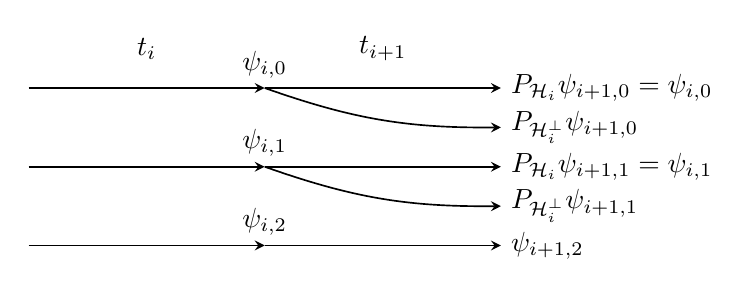
\begin{tikzpicture}[>=stealth, semithick]
        \node at (1.5, 0) {\(t_i\)};
        \draw[->] (0, -0.5) -- (3, -0.5) node[above] {\(\ket{\psi_{i, 0}}\)};
        \draw[->] (3, -0.5) -- (6, -0.5) node[right] {\(P_{\mathcal{H}_i}\ket{\psi_{i+1, 0}} = \ket{\psi_{i, 0}}\)};
        \draw (3, -0.5) edge[->, bend right=10] node[pos=1.0, right] {\(P_{\mathcal{H}_{i}^\perp} \ket{\psi_{i+1, 0}}\)} (6, -1.0);
        \draw[->] (0, -1.5) -- (3, -1.5) node[above] {\(\ket{\psi_{i, 1}}\)};
        \draw[->] (3, -1.5) -- (6, -1.5) node[right] {\(P_{\mathcal{H}_i}\ket{\psi_{i+1, 1}} = \ket{\psi_{i, 1}}\)};
        \draw (3, -1.5) edge[->, bend right=10] node[pos=1.0, right] {\(P_{\mathcal{H}_{i}^\perp} \ket{\psi_{i+1, 1}}\)} (6, -2.0);
        \draw[->] (0, -2.5) -- (3, -2.5) node[above] {\(\ket{\psi_{i, 2}}\)};
        \draw[->] (3, -2.5) -- (6, -2.5) node[right] {\(\ket{\psi_{i+1, 2}}\)};
        \node at (4.5, 0) {\(t_{i+1}\)};
    \end{tikzpicture}
    \caption{Illustation of the difference between the three components of two different consecutive states in a VTAA algorithm, where \(i \in [1, m]_{\mathbb{N}}\) is fixed. The branches in the arrows indicate sums, i.e. e.g. \(\ket{\psi_{i, 0}} = P_{\mathcal{H}_i}\ket{\psi_{i, 0}} + P_{\mathcal{H}_i^\perp}\ket{\psi_{i, 0}}.\)}
    \label{vtaa_illustration}
\end{figure}

The times \(t_1, ..., t_m\) and probabilities \(p_1, ..., p_m\) were let lose by us and are up to the algorithm designer to choose. As Ambainis, one may define the \emph{average stopping time} by
\begin{align}
    T_a \coloneqq \sqrt{\sum_{i=1}^m p_i t_i^2}
\end{align}
and set the maximum time \(T_M \coloneqq t_m\) and the success probability at time point \(t_m\) to be \(p_s \coloneqq |\alpha_{m, 1}|^2\). Ambainis then proves the following theorem.

\begin{theorem}
    There is a quantum algorithm, which amplifies the success probability of an algorithm in the VTAA model to give a successful measurement in time
    \begin{align}
        \onot\left(T_M\log^{0.5}(T_M)+\frac{T_a}{p_s}\log^{1.5}(T_M)\right)
    \end{align}
\end{theorem}

The main result by Ambainis is now, that by expressing the HHL algorithm inside of the VTAA model, we can improve the success probability from \(\onot(\kappa^2)\) wrt. the runtime factor of \(\kappa\). There we had \(\onot(\kappa^2)\) as the dependence, which was obtained by choosing the evolution time in dependence of \(\onot(\kappa)\) and then running AA for another dependence on \(\onot(\kappa)\). Ambainis acquires the following result \cite[pp. 8-12]{Ambainis2010}.

\begin{theorem}
    Using VTAA, there is a quantum algorithm, which improves the runtime of the HHL algorithm to
    \begin{align}
        \tilde{\onot}\left(\log_2(N) \kappa \log_2^3\left(\frac{\kappa}{\varepsilon}\right) s^2 \log_2^2\left(\frac{1}{\varepsilon}\right) \frac{1}{\varepsilon^3}\right)
    \end{align}
\end{theorem}

The runtime cited comes from the fact, that the phase estimation procedure of runtime \(\onot(\log_2(N) \kappa s^2 / \varepsilon)\) is used as a subprocedure of the algorithm \cite[p. 9]{Ambainis2010}, but Ambainis omits the \(\onot(\log_2(N) s^2)\) factor in \cite[p. 12]{Ambainis2010}. Note, that we cited the runtime factor \(\onot(s^2)\) to conform with these papers, although it should be \(\onot(s^4)\).

\begin{remark}
    We may note, that while the dependence on \(\kappa\) is better than the original HHL algorithm, the error dependence is significantly worse.
\end{remark}

\paragraph*{Fourier Decompositions for Sublinear Error Dependence} \label{hhl_fourier_approach} \phantom{}\\\phantom{}

In a 2015 paper, Childs et al. presented three approaches \cite{Childs2015} to substantially improving the error dependence of the HHL algorithm. We shortly describe the so-called \emph{Fourier approach}, which we shall divide into the explanation of three conceptual steps.

\begin{itemize}
    \item First, the results include the use of newer techniques for the Hamiltonian simulation, as presented by Childs et al. in \cite{Berry2015}.
    \item Secondly, one important aspect of the paper is the use of LCUs as in \cite[pp. 5-8]{Childs2015}. Let \(A \in \mathbb{C}^{N \times N}, N \coloneqq 2^n, n \in \mathbb{N}_{\geq 1}\) be the matrix of the SLE. Assume further it is, possibly after a reduction, Hermitian and assume for the sake of the conceptual overview, that it is invertible. The idea is then to, similiarly to the Hamiltonian decomposition in \Cref{hamiltonian_simulation}, decompose the matrix \(A^{-1}\) into a unitary sum and to simulate the sum. The unitaries chosen are indeed \(e^{iAt_j}\), where \(t_j \in \mathbb{R}\) are times, giving a decomposition of form \(A^{-1} = \sum_{j}\alpha_je^{iAt_j}\) with coefficients \(\alpha_j \in \mathbb{C}\). By performing a basis switch, the authors then reduce the problem of approximating this decomposition to approximating a real univariate decomposition \(x^{-1} = \sum_j \alpha_j e^{ixt_j}\) for \(x \in [-1, -1/\kappa] \cup [1/\kappa, 1]\).
    \item Thirdly, to compute the aforementioned decomposition of \(1/x\), the following Fourier transformation is used:
    \begin{align}
        \frac{1}{x} = \frac{i}{\sqrt{2\pi}}\int_0^\infty\int_{-\infty}^\infty ze^{-z^2/2}e^{-ixyz} \; dz \; dy
    \end{align}
    As in \cite[pp. 10-11]{Childs2015}. It is shown how to discretize these integrals, giving a suitable quantum algorithm for approximating \(A^{-1}\).
\end{itemize}
We recognize again the pattern of using an efficient decomposition of the initial linear operator for solving the SLE problem. Childs et al. then have as one of their results the following theorem as in \cite[p. 4]{Childs2015}.
\begin{theorem}[Fourier Approach to HHL]
    Using more recent results for Hamiltonian simulation, techniques involving LCUs and Fourier transformations, there is a quantum algorithm for solving an SLE in time
    \begin{align}
        \onot\left(s\kappa^2\log_2^{2.5}\left(\frac{\kappa}{\varepsilon}\right)\left(\log_2(N)+\log_2^{2.5}\left(\frac{\kappa}{\varepsilon}\right)\right)\right)
    \end{align}
\end{theorem}

The other two approaches include the use of \emph{Chebyshev polynomials} and the modification of Ambainis' VTAA HHL algorithm. The three approaches are not equivalent, as pointed out in \cite[p. 4]{Childs2015} and have their own advantages and disadvantages, which we shall not elaborate, as this is a high level overview of the results.
